% Created 2019-12-10 Tue 10:47
% Intended LaTeX compiler: pdflatex
\documentclass[10pt, compress, aspectratio=169, xcolor={table,usenames,dvipsnames}]{beamer}

\usepackage{booktabs}
\mode<beamer>{\usetheme[numbering=fraction, progressbar=none, titleformat=smallcaps, sectionpage=none]{metropolis}}
\usepackage{sourcecodepro}
\usepackage{booktabs}
\usepackage{array}
\usepackage{listings}
\usepackage{graphicx}
\usepackage[english]{babel}
\usepackage[scale=2]{ccicons}
\usepackage{url}
\usepackage{relsize}
\usepackage{amsmath}
\usepackage{bm}
\usepackage{wasysym}
\usepackage{ragged2e}
\usepackage{textcomp}
\usepackage{pgfplots}
\usepackage{multirow}
\usepgfplotslibrary{dateplot}
\definecolor{Base}{HTML}{191F26}
\definecolor{Highlight}{HTML}{ffda99}
\definecolor{Accent}{HTML}{bb0300}
\setbeamercolor{alerted text}{fg=Accent}
\setbeamercolor{frametitle}{bg=Base}
\setbeamercolor{normal text}{bg=black!2,fg=Base}
\setsansfont[BoldFont={Source Sans Pro Semibold},Numbers={OldStyle}]{Source Sans Pro}
\lstdefinelanguage{Julia}%
{morekeywords={abstract,struct,break,case,catch,const,continue,do,else,elseif,%
end,export,false,for,function,immutable,mutable,using,import,importall,if,in,%
macro,module,quote,return,switch,true,try,catch,type,typealias,%
while,<:,+,-,::,/},%
sensitive=true,%
alsoother={$},%
morecomment=[l]\#,%
morecomment=[n]{\#=}{=\#},%
morestring=[s]{"}{"},%
morestring=[m]{'}{'},%
}[keywords,comments,strings]%
\lstset{ %
backgroundcolor={},
basicstyle=\ttfamily\scriptsize,
breakatwhitespace=true,
breaklines=true,
captionpos=n,
commentstyle=\color{Accent},
extendedchars=true,
frame=n,
keywordstyle=\color{Accent},
language=R,
rulecolor=\color{black},
showspaces=false,
showstringspaces=false,
showtabs=false,
stepnumber=2,
stringstyle=\color{gray},
tabsize=2,
}
\renewcommand*{\UrlFont}{\ttfamily\smaller\relax}
\graphicspath{{../../img/}}
\addtobeamertemplate{block begin}{}{\justifying}
\usetheme{default}
\author{ \footnotesize \textbf{\alert{Pedro Bruel}},  Steven Quinito Masnada, Brice Videau, Arnaud Legrand, Jean-Marc Vincent, Alfredo Goldman}
\date{ \scriptsize \textit{phrb@ime.usp.br} \\[1em] \textit{Université Grenoble Alpes, France} \\ \textit{Universidade de São Paulo, Brazil}}
\title{Autotuning under Tight Budget Constraints:  \\ An Experimental Design Approach}
\hypersetup{
 pdfauthor={ \footnotesize \textbf{\alert{Pedro Bruel}},  Steven Quinito Masnada, Brice Videau, Arnaud Legrand, Jean-Marc Vincent, Alfredo Goldman},
 pdftitle={Autotuning under Tight Budget Constraints:  \\ An Experimental Design Approach},
 pdfkeywords={},
 pdfsubject={},
 pdfcreator={Emacs 26.3 (Org mode 9.2.5)},
 pdflang={English}}
\begin{document}

\maketitle

\section{Autotuning}
\label{sec:org4e6596b}
\begin{frame}[label={sec:orgcc55431}]{Autotuning: Optimizing Program Configurations}
\begin{columns}
\begin{column}{0.5\columnwidth}
\begin{block}{Architectures for High Performance Computing}
\begin{center}
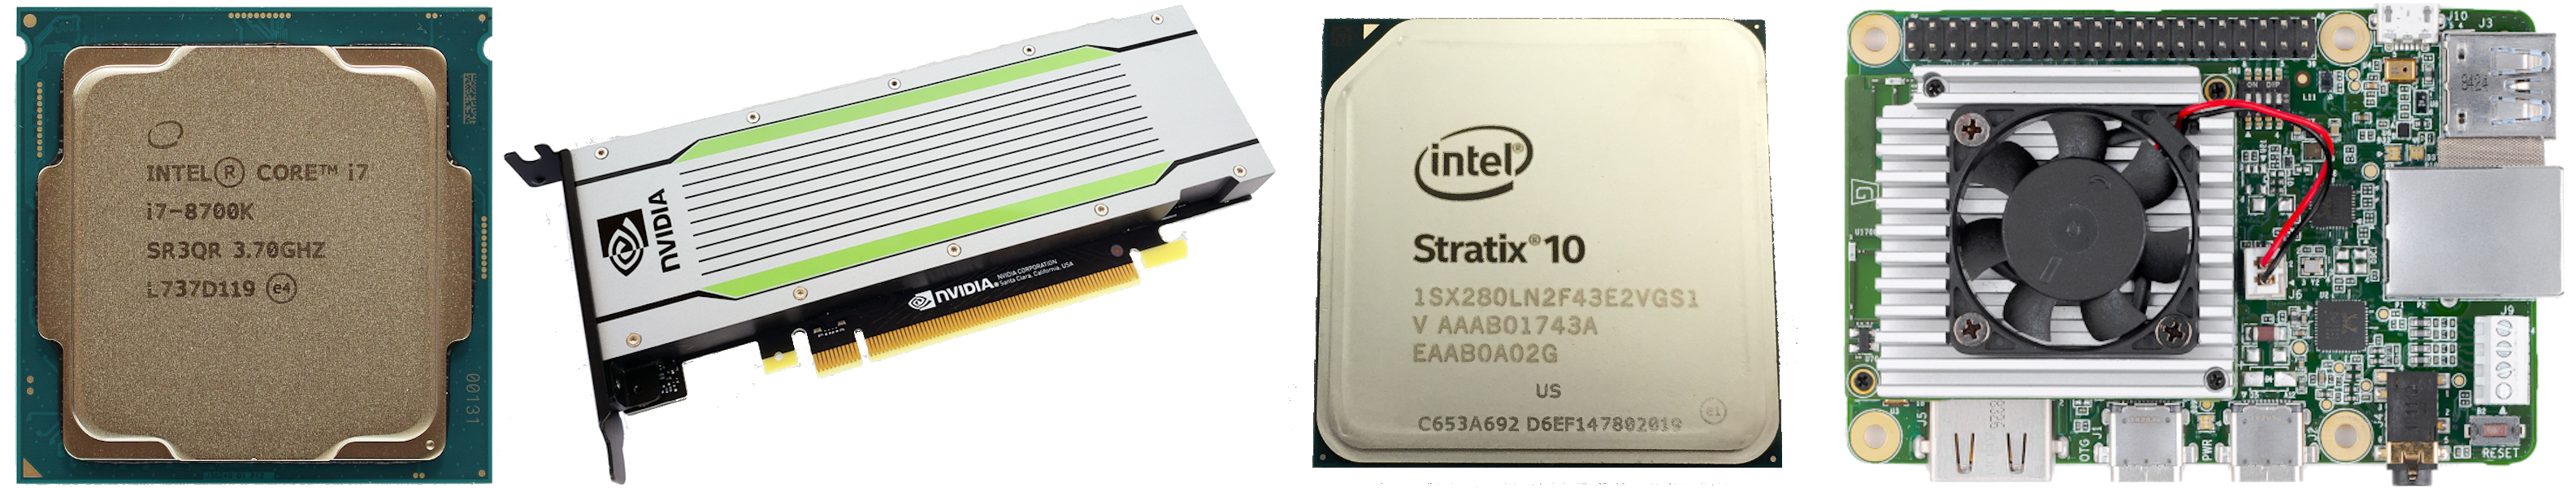
\includegraphics[width=\columnwidth]{../../../img/architectures_2.png}
\end{center}

How to write \alert{efficient code} for each of these?

\begin{block}{Autotuning}
\vspace{.2cm}

The process of automatically finding a \mbox{\alert{configuration}} of a program
that optimizes an \mbox{\alert{objective}}
\end{block}
\end{block}
\end{column}

\begin{column}{0.5\columnwidth}
\begin{block}{Configurations}
\begin{itemize}
\item Algorithms
\begin{itemize}
\item Sorting, encoding, \(\dots\)
\end{itemize}
\item Implementations
\begin{itemize}
\item Code transformation, libraries, \(\dots\)
\end{itemize}
\item Context-specific parameters
\begin{itemize}
\item Compilers, kernels, \(\dots\)
\end{itemize}
\end{itemize}

\begin{block}{Objectives}
\begin{itemize}
\item Execution time
\item Resource consumption
\item Binary size
\item \(\dots\)
\end{itemize}
\end{block}
\end{block}
\end{column}
\end{columns}
\end{frame}

\begin{frame}[label={sec:org65cca3f}]{Autotuning: Search Spaces}
\begin{columns}
\begin{column}{0.4\columnwidth}
\begin{block}{Search Spaces}
\vspace{.2cm}

Represent the \alert{effect} of all possible
configurations on target objectives

Can be difficult to explore, with multiple \mbox{\alert{local optima}}
and \mbox{\alert{undefined}} \mbox{\alert{regions}}
\end{block}
\end{column}

\begin{column}{0.6\columnwidth}
\begin{center}
\begin{center}
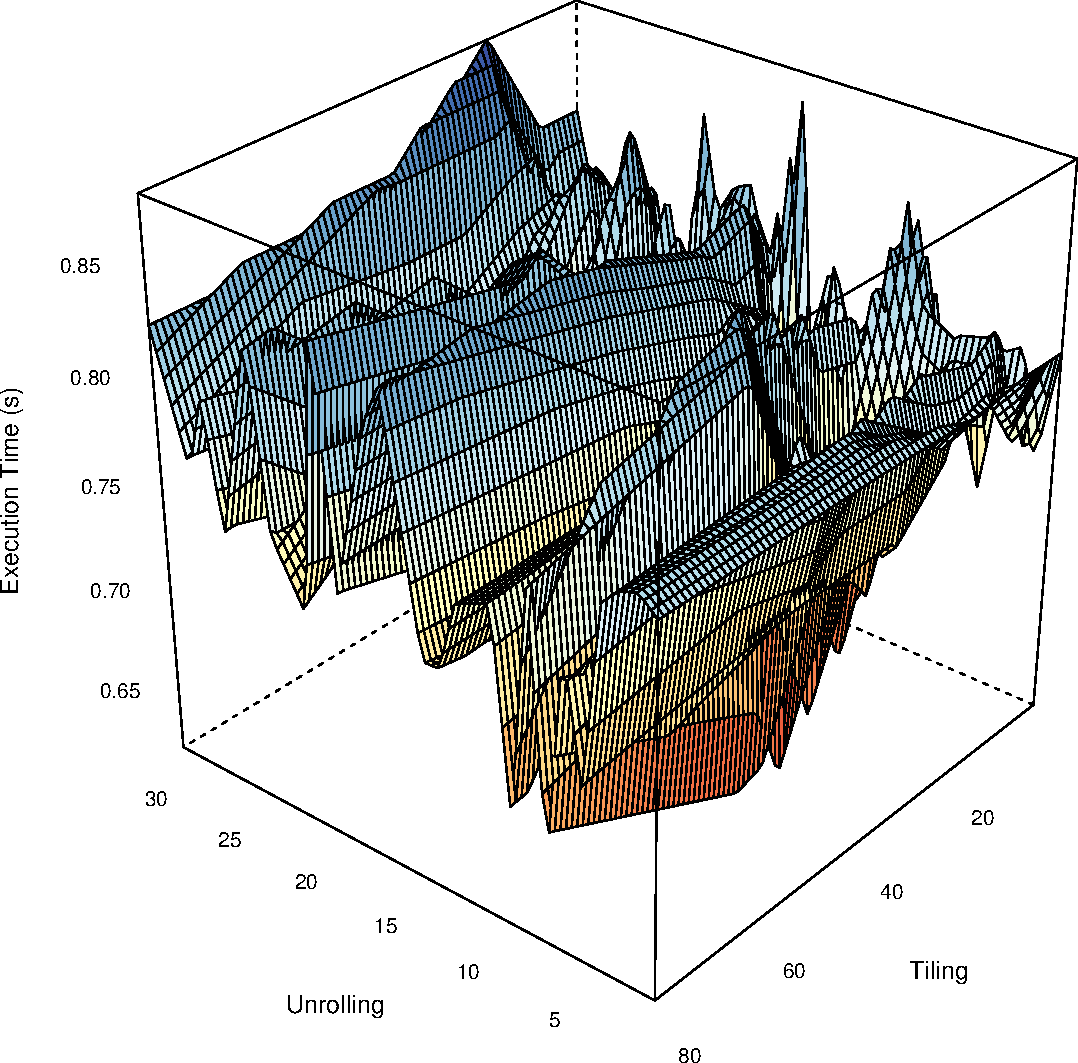
\includegraphics[width=.8\columnwidth]{../../../img/bicgkernel_averaged_search_space.pdf}
\end{center}
\end{center}

\center{\footnotesize
Unrolling, tiling and performance for a \alert{biconjugate gradient} kernel
}
\end{column}
\end{columns}
\end{frame}

\begin{frame}[label={sec:org959a820}]{Autotuning: High-Dimensional Search Spaces}
\begin{block}{1. \alert{Combinatorial Explosion \& Sampling}}
\begin{itemize}
\item 10 boolean parameters generate \(2^{10}\) combinations
\item 10 continuous parameters in \([0, 1]\)  need \((10^{2})^{10}\) points to cover with
spacing \(10^{-2}\)
\item Sampling a hypercube covers its shell
\end{itemize}
\end{block}

\begin{columns}
\begin{column}{0.5\columnwidth}
\begin{block}{2. \alert{Geometry}}
\begin{itemize}
\item Mixing numerical and categorical factors
\item ``Smoothness''
\item Interactions
\item Constraints
\item Undefined regions
\end{itemize}
\end{block}
\end{column}

\begin{column}{0.5\columnwidth}
\begin{block}{3. \alert{Measurement Time}}
\begin{itemize}
\item Compile time:
\begin{itemize}
\item FPGA applications
\item Hardware/Software codesign
\end{itemize}
\item Execution time:
\begin{itemize}
\item Simulations
\item Neural network training
\end{itemize}
\end{itemize}
\end{block}
\end{column}
\end{columns}
\end{frame}

\begin{frame}[label={sec:orga11c9e0}]{Autotuning: Approaches}
\begin{columns}
\begin{column}{0.5\columnwidth}
\begin{block}{Several Approaches}
\footnotesize
\begin{itemize}
\item \colorbox{red!25}{Exhaustive}
\item \colorbox{green!25}{Meta-Heuristics}
\item \colorbox{cyan!25}{Machine Learning}
\end{itemize}
\normalsize

\vspace{-.4cm}

\begin{table}
    \centering
    \scriptsize
    \begin{tabular}{@{}lll@{}}
        \toprule
        System & Domain & Approach \\ \midrule
        \rowcolor{red!25} ATLAS & Dense Linear Algebra & Exhaustive\\ \addlinespace
        \rowcolor{green!25} INSIEME & Compiler & Genetic Algorithm \\
        \rowcolor{green!25} Active Harmony & Runtime & Nelder-Mead \\
        \rowcolor{green!25} ParamILS & Domain-Agnostic & Stochastic Local Search \\
        \rowcolor{green!25} OPAL & Domain-Agnostic & Direct Search \\
        \rowcolor{green!25} OpenTuner & Domain-Agnostic & Ensemble \\ \addlinespace
        \rowcolor{cyan!25} MILEPOST GCC & Compiler & Machine Learning \\
        \rowcolor{cyan!25} Apollo & GPU kernels & Decision Trees \\ \addlinespace
        \bottomrule
    \end{tabular}
\end{table}

\end{block}
\end{column}

\begin{column}{0.5\columnwidth}
\begin{block}{Core Assumptions:}
\begin{itemize}
\item A large number of function evaluations
\item Good solutions are reachable
\item Seach space ``smoothness''
\end{itemize}
\begin{block}{After Optimization:}
\begin{itemize}
\item \alert{Learn ``nothing''} about the search space
\item \alert{Can't explain} why optimizations work
\end{itemize}
\end{block}
\begin{block}{We propose using:}
\begin{itemize}
\item \alert{Experimental Design} (\alert{ED}), or \alert{Design of Experiments} (\alert{DoE})
\end{itemize}
\end{block}
\end{block}
\end{column}
\end{columns}
\end{frame}
\section{Experimental Design}
\label{sec:org837dc13}
\begin{frame}[label={sec:org642ea60}]{Experimental Design: An Example on Agriculture}
\begin{columns}
\begin{column}{0.55\columnwidth}
\begin{center}
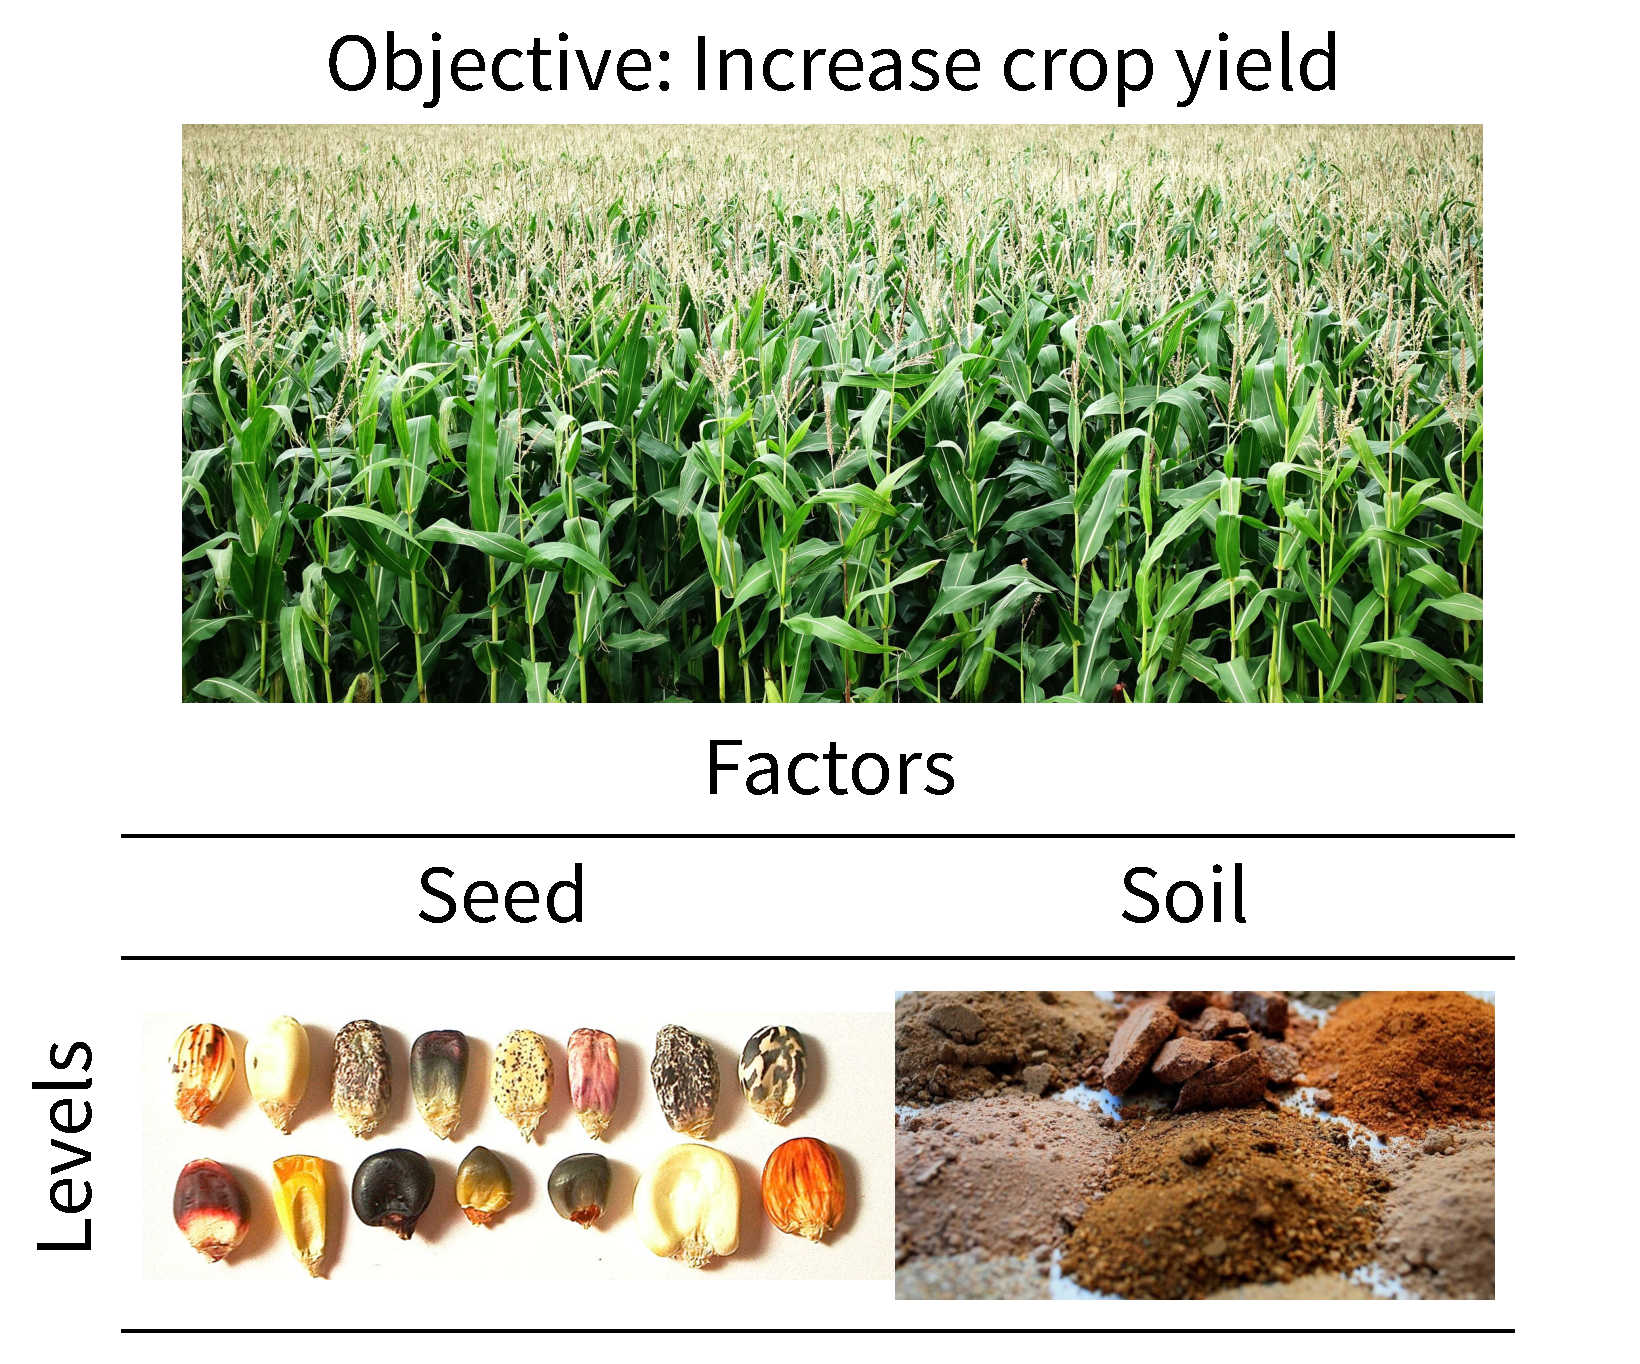
\includegraphics[width=.99\columnwidth]{../../../img/crop_yield_doe_example.pdf}
\end{center}
\end{column}
\begin{column}{0.45\columnwidth}
\begin{block}{Testing all combinations is \alert{inviable}}
\begin{block}{Which combinations to test?}
\begin{itemize}
\item ED provides a selection method
\item \colorbox{Highlight}{\alert{Parsimony}: decreases experiments}
\end{itemize}
\end{block}

\begin{block}{Which is the best combination?}
\begin{itemize}
\item ED provides an analysis method
\item \colorbox{Highlight}{\alert{Transparency}: use statistical tests}
\end{itemize}
\end{block}
\end{block}
\end{column}
\end{columns}
\end{frame}

\begin{frame}[label={sec:org8314b39}]{Experimental Design}
\begin{columns}
\begin{column}{0.5\columnwidth}
\begin{block}{Terminology}
\begin{itemize}
\item Factors: program parameters
\item Levels: possible factor values
\item Experiment: setting each factor to a level
\item Design: a selection of experiments to run
\item \uncover<2>{Performance model: guides selection}
\end{itemize}

\begin{block}{Analyzing Results Enables:}
\begin{itemize}
\item Identifying \alert{significant factors}
\item Finding \alert{candidates} for further exploration
\item Investigating possible \alert{models}
\end{itemize}
\end{block}
\end{block}
\end{column}

\begin{column}{0.5\columnwidth}
\begin{block}{Example}
\vspace{-.2cm}
\begin{center}

A minimal screening design for \(7\) 2-level factors:

\end{center}
\vspace{-.2cm}

\only<1>{
\begin{table}[]
    \centering
    \begin{tabular}{@{\kern\tabcolsep}cccccccc@{\kern\tabcolsep}}
        \toprule
        Run & A & B & C & D & E & F & G \\ \midrule
        \cellcolor{gray!18}1 & \cellcolor{green!25}1 & \cellcolor{red!25}-1 & \cellcolor{green!25}1 & \cellcolor{red!25}-1 & \cellcolor{red!25}-1 & \cellcolor{green!25}1 & \cellcolor{green!25}1 \\
        \cellcolor{gray!18}2 & \cellcolor{green!25}1 & \cellcolor{green!25}1 & \cellcolor{green!25}1 & \cellcolor{red!25}-1 & \cellcolor{green!25}1 & \cellcolor{red!25}-1 & \cellcolor{red!25}-1 \\
        \cellcolor{gray!18}3 & \cellcolor{red!25}-1 & \cellcolor{green!25}1 & \cellcolor{red!25}-1 & \cellcolor{red!25}-1 & \cellcolor{green!25}1 & \cellcolor{green!25}1 & \cellcolor{green!25}1 \\
        \cellcolor{gray!18}4 & \cellcolor{red!25}-1 & \cellcolor{green!25}1 & \cellcolor{green!25}1 & \cellcolor{green!25}1 & \cellcolor{red!25}-1 & \cellcolor{green!25}1 & \cellcolor{red!25}-1 \\
        \cellcolor{gray!18}5 & \cellcolor{green!25}1 & \cellcolor{red!25}-1 & \cellcolor{red!25}-1 & \cellcolor{green!25}1 & \cellcolor{green!25}1 & \cellcolor{green!25}1 & \cellcolor{red!25}-1 \\
        \cellcolor{gray!18}6 & \cellcolor{green!25}1 & \cellcolor{green!25}1 & \cellcolor{red!25}-1 & \cellcolor{green!25}1 & \cellcolor{red!25}-1 & \cellcolor{red!25}-1 & \cellcolor{green!25}1 \\
        \cellcolor{gray!18}7 & \cellcolor{red!25}-1 & \cellcolor{red!25}-1 & \cellcolor{green!25}1 & \cellcolor{green!25}1 & \cellcolor{green!25}1 & \cellcolor{red!25}-1 & \cellcolor{green!25}1 \\
        \cellcolor{gray!18}8 & \cellcolor{red!25}-1 & \cellcolor{red!25}-1 & \cellcolor{red!25}-1 & \cellcolor{red!25}-1 & \cellcolor{red!25}-1 & \cellcolor{red!25}-1 & \cellcolor{red!25}-1  \\ \bottomrule
    \end{tabular}
\end{table}

}
\only<2>{
\begin{table}[]
    \centering
    \begin{tabular}{@{\kern\tabcolsep}ccccccccc@{\kern\tabcolsep}}
        \toprule
        Run & $\theta$ & A & B & C & D & E & F & G \\ \midrule
        \cellcolor{gray!18}1 & \cellcolor{blue!12}1 & \cellcolor{green!25}1 & \cellcolor{red!25}-1 & \cellcolor{green!25}1 & \cellcolor{red!25}-1 & \cellcolor{red!25}-1 & \cellcolor{green!25}1 & \cellcolor{green!25}1 \\
        \cellcolor{gray!18}2 & \cellcolor{blue!12}1 & \cellcolor{green!25}1 & \cellcolor{green!25}1 & \cellcolor{green!25}1 & \cellcolor{red!25}-1 & \cellcolor{green!25}1 & \cellcolor{red!25}-1 & \cellcolor{red!25}-1 \\
        \cellcolor{gray!18}3 & \cellcolor{blue!12}1 & \cellcolor{red!25}-1 & \cellcolor{green!25}1 & \cellcolor{red!25}-1 & \cellcolor{red!25}-1 & \cellcolor{green!25}1 & \cellcolor{green!25}1 & \cellcolor{green!25}1 \\
        \cellcolor{gray!18}4 & \cellcolor{blue!12}1 & \cellcolor{red!25}-1 & \cellcolor{green!25}1 & \cellcolor{green!25}1 & \cellcolor{green!25}1 & \cellcolor{red!25}-1 & \cellcolor{green!25}1 & \cellcolor{red!25}-1 \\
        \cellcolor{gray!18}5 & \cellcolor{blue!12}1 & \cellcolor{green!25}1 & \cellcolor{red!25}-1 & \cellcolor{red!25}-1 & \cellcolor{green!25}1 & \cellcolor{green!25}1 & \cellcolor{green!25}1 & \cellcolor{red!25}-1 \\
        \cellcolor{gray!18}6 & \cellcolor{blue!12}1 & \cellcolor{green!25}1 & \cellcolor{green!25}1 & \cellcolor{red!25}-1 & \cellcolor{green!25}1 & \cellcolor{red!25}-1 & \cellcolor{red!25}-1 & \cellcolor{green!25}1 \\
        \cellcolor{gray!18}7 & \cellcolor{blue!12}1 & \cellcolor{red!25}-1 & \cellcolor{red!25}-1 & \cellcolor{green!25}1 & \cellcolor{green!25}1 & \cellcolor{green!25}1 & \cellcolor{red!25}-1 & \cellcolor{green!25}1 \\
        \cellcolor{gray!18}8 & \cellcolor{blue!12}1 & \cellcolor{red!25}-1 & \cellcolor{red!25}-1 & \cellcolor{red!25}-1 & \cellcolor{red!25}-1 & \cellcolor{red!25}-1 & \cellcolor{red!25}-1 & \cellcolor{red!25}-1  \\ \bottomrule
    \end{tabular}
\end{table}

}
\vspace{-.2cm}

\uncover<2>{$$response = \theta{} + \alpha{}A + \beta{}B + \gamma{}C + \dots$$}
\end{block}
\end{column}
\end{columns}
\end{frame}

\begin{frame}[label={sec:org2d01443}]{Applying Experimental Design to Autotuning}
\begin{columns}
\begin{column}{0.45\columnwidth}
\begin{block}{Design Requirements}
\begin{itemize}
\item Support a large number of factors (\alert{Combinatorial Explosion})
\item Maximize the amount of information (\alert{Sampling})
\item Support mixing factor types (\alert{Geometry})
\item Minimize function evaluations (\alert{Measurement Time})
\end{itemize}
\end{block}
\end{column}

\begin{column}{0.55\columnwidth}
\begin{block}{Initial Experimental Design Approach}
\begin{itemize}
\item \colorbox{Highlight}{\alert{Parsimony} \& \alert{Transparency}}
\item \alert{D-Optimal} designs
\begin{itemize}
\item Flexible
\item Minimize variance of coefficient estimators
\item Support different factor types
\end{itemize}
\item \alert{Linear model} and analysis of variance (\alert{ANOVA})
\item User input to guide optimization
\end{itemize}

\begin{block}{Validation}
\begin{itemize}
\item Code transformation:
\begin{itemize}
\item GPU Laplacian kernel
\item HPC kernels from the SPAPT benchmark
\end{itemize}
\end{itemize}
\end{block}
\end{block}
\end{column}
\end{columns}
\end{frame}

\begin{frame}[label={sec:orgcfc28a7}]{D-Optimal Designs: A Simple Example in R}
\begin{columns}
\begin{column}{0.5\columnwidth}
\begin{block}{Search Space}
\begin{itemize}
\item Factors \& Levels:
\begin{align*}
\mathbf{X} = x_i \in (x_{i,1} \in & \; (1, 2, 3, 4, 5), \\
x_{i,2} \in & \; (``A", ``B", ``C"))
\end{align*}
\item 15 possible experiments
\item Model: \(\mathbf{Y} = \mathbf{X}\bm{\beta} + \bm{\varepsilon}\)
\end{itemize}
\end{block}
\end{column}

\begin{column}{0.5\columnwidth}
\begin{block}{Ordinary Least Squares Estimator \(\bm{\hat{\beta}}\)}
\begin{center}
\begin{equation*}
\bm{\hat{\beta}} = \left(\bm{X}^{\intercal}\bm{X}\right)^{-1}\bm{X}^{\intercal}\bm{Y}
\end{equation*}
\end{center}

\begin{center}
\colorbox{Highlight}{\parbox[c]{0.8\columnwidth}{\centering   The  variance   of
    $\bm{\hat{\beta}}$  is  \alert{proportional}  to \\  the  covariance  matrix
    $\left(\bm{X}^{\intercal}\bm{X}\right)^{-1}$}}

\pause

\colorbox{Highlight}{\parbox[c]{0.8\columnwidth}{\centering   We   can   improve
    $\bm{\hat{\beta}}$ \\ \alert{without knowledge} of $\bm{Y}$}}
\end{center}
\end{block}
\end{column}
\end{columns}
\end{frame}

\begin{frame}[label={sec:org2db987f},fragile]{D-Optimal Designs: A Simple Example in R}
 \begin{columns}
\begin{column}{0.7\columnwidth}
\begin{block}{Source code in \texttt{R}}
\vspace{-.2cm}

\lstset{language=r,label= ,caption= ,captionpos=b,numbers=none}
\begin{lstlisting}
library(DoE.base)
library(AlgDesign)

samples <- fac.design(nfactors = 2,
                      nlevels = c(5, 3),
                      factor.names = list(x1 = 1:5,
                                          x2 = c("A", "B", "C")))

output <- optFederov(~ x1 + x2,
                     samples,
                     nTrials = 7)
\end{lstlisting}

\begin{block}{Optimality Criteria on \(\left(\bm{X}^{\intercal}\bm{X}\right)^{-1}\)}
\begin{itemize}
\item \alert{D}: minimizes the determinant
\item \alert{A}: minimizes the trace
\item \dots{}
\end{itemize}
\end{block}
\end{block}
\end{column}


\begin{column}{0.3\columnwidth}
\begin{block}{Output}
\vspace{-.2cm}
\scriptsize

\begin{verbatim}
$D
[1] 0.1797856

$design
   x1 x2
4   5  A
5   4  A
7   3  A
9   2  A
10  1  A
11  3  C
13  1  B
\end{verbatim}


\normalsize
\end{block}
\end{column}
\end{columns}
\end{frame}

\begin{frame}[label={sec:org63e16d9}]{Comparing Sampling Strategies: \(z = \theta + x + x^2 + y + y^2 + \varepsilon\)}
\begin{center}
\begin{center}
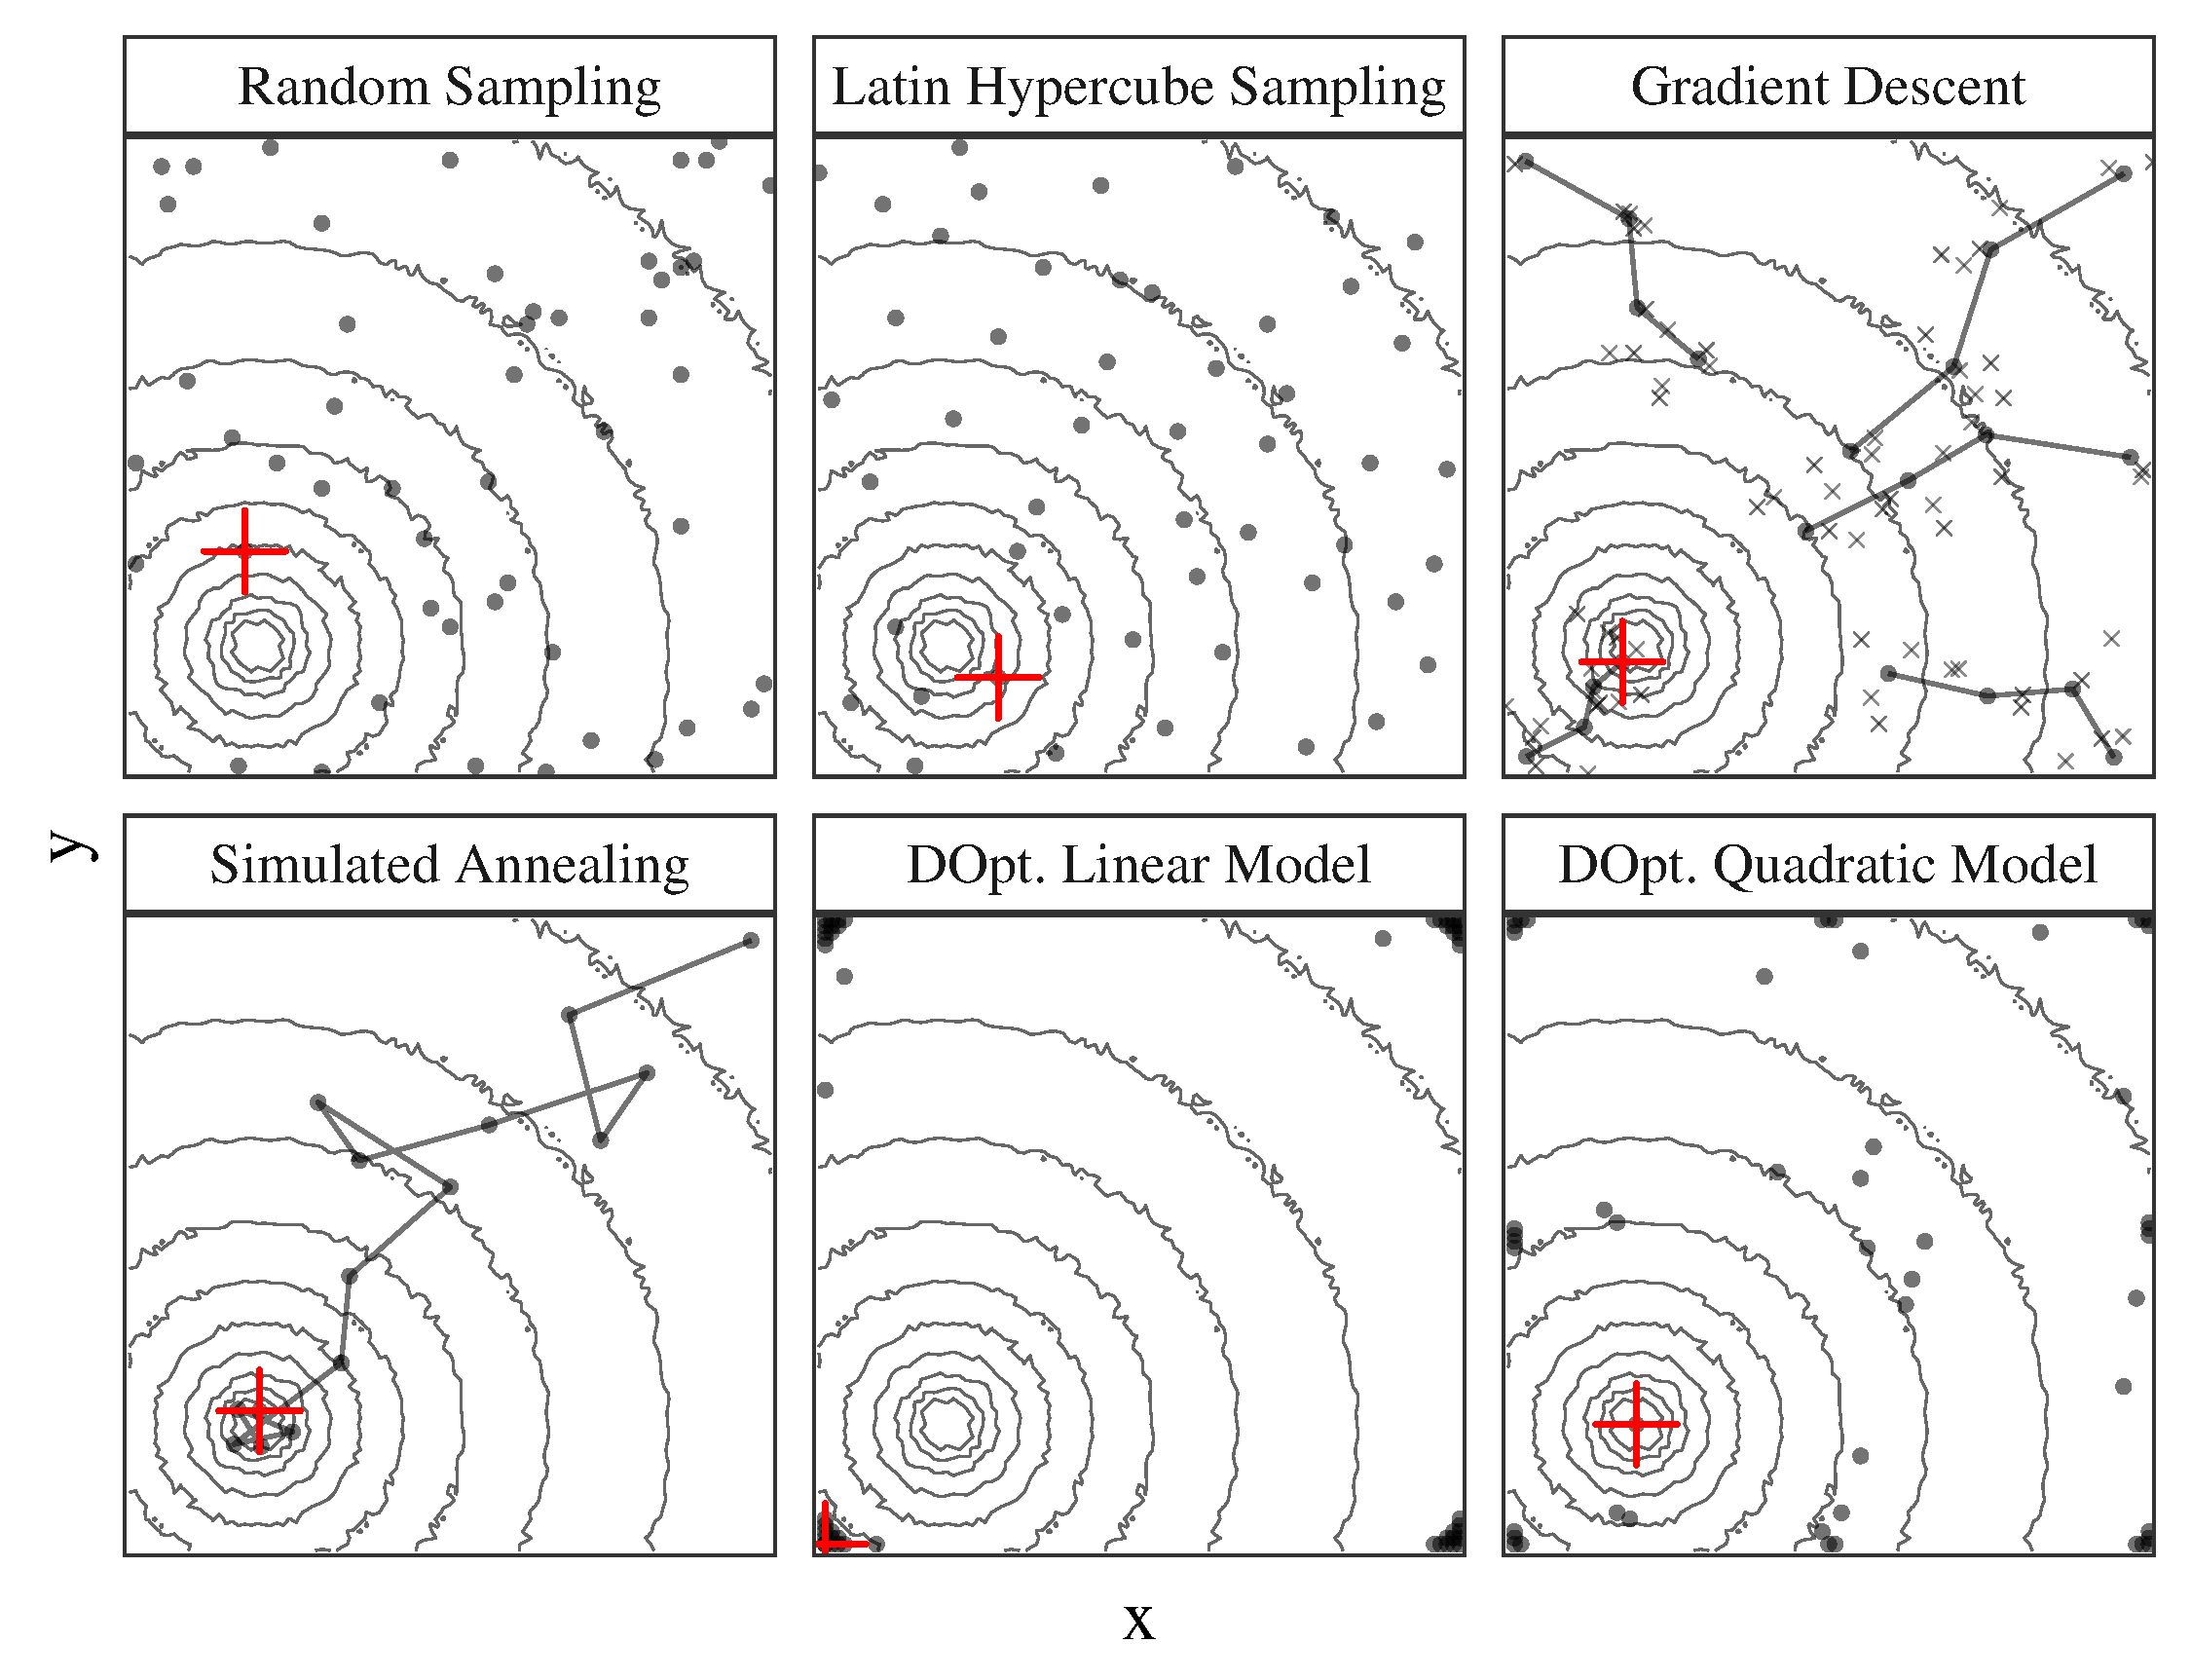
\includegraphics[width=.72\textwidth]{../../../img/sampling_comparison.pdf}
\end{center}
\end{center}
\end{frame}
\section{A Transparent and Parsimonious ED Approach to Autotuning}
\label{sec:org1e115fb}
\begin{frame}[label={sec:orgd40fd99}]{A Experimental Design Approach to Autotuning}
\begin{center}
\begin{center}
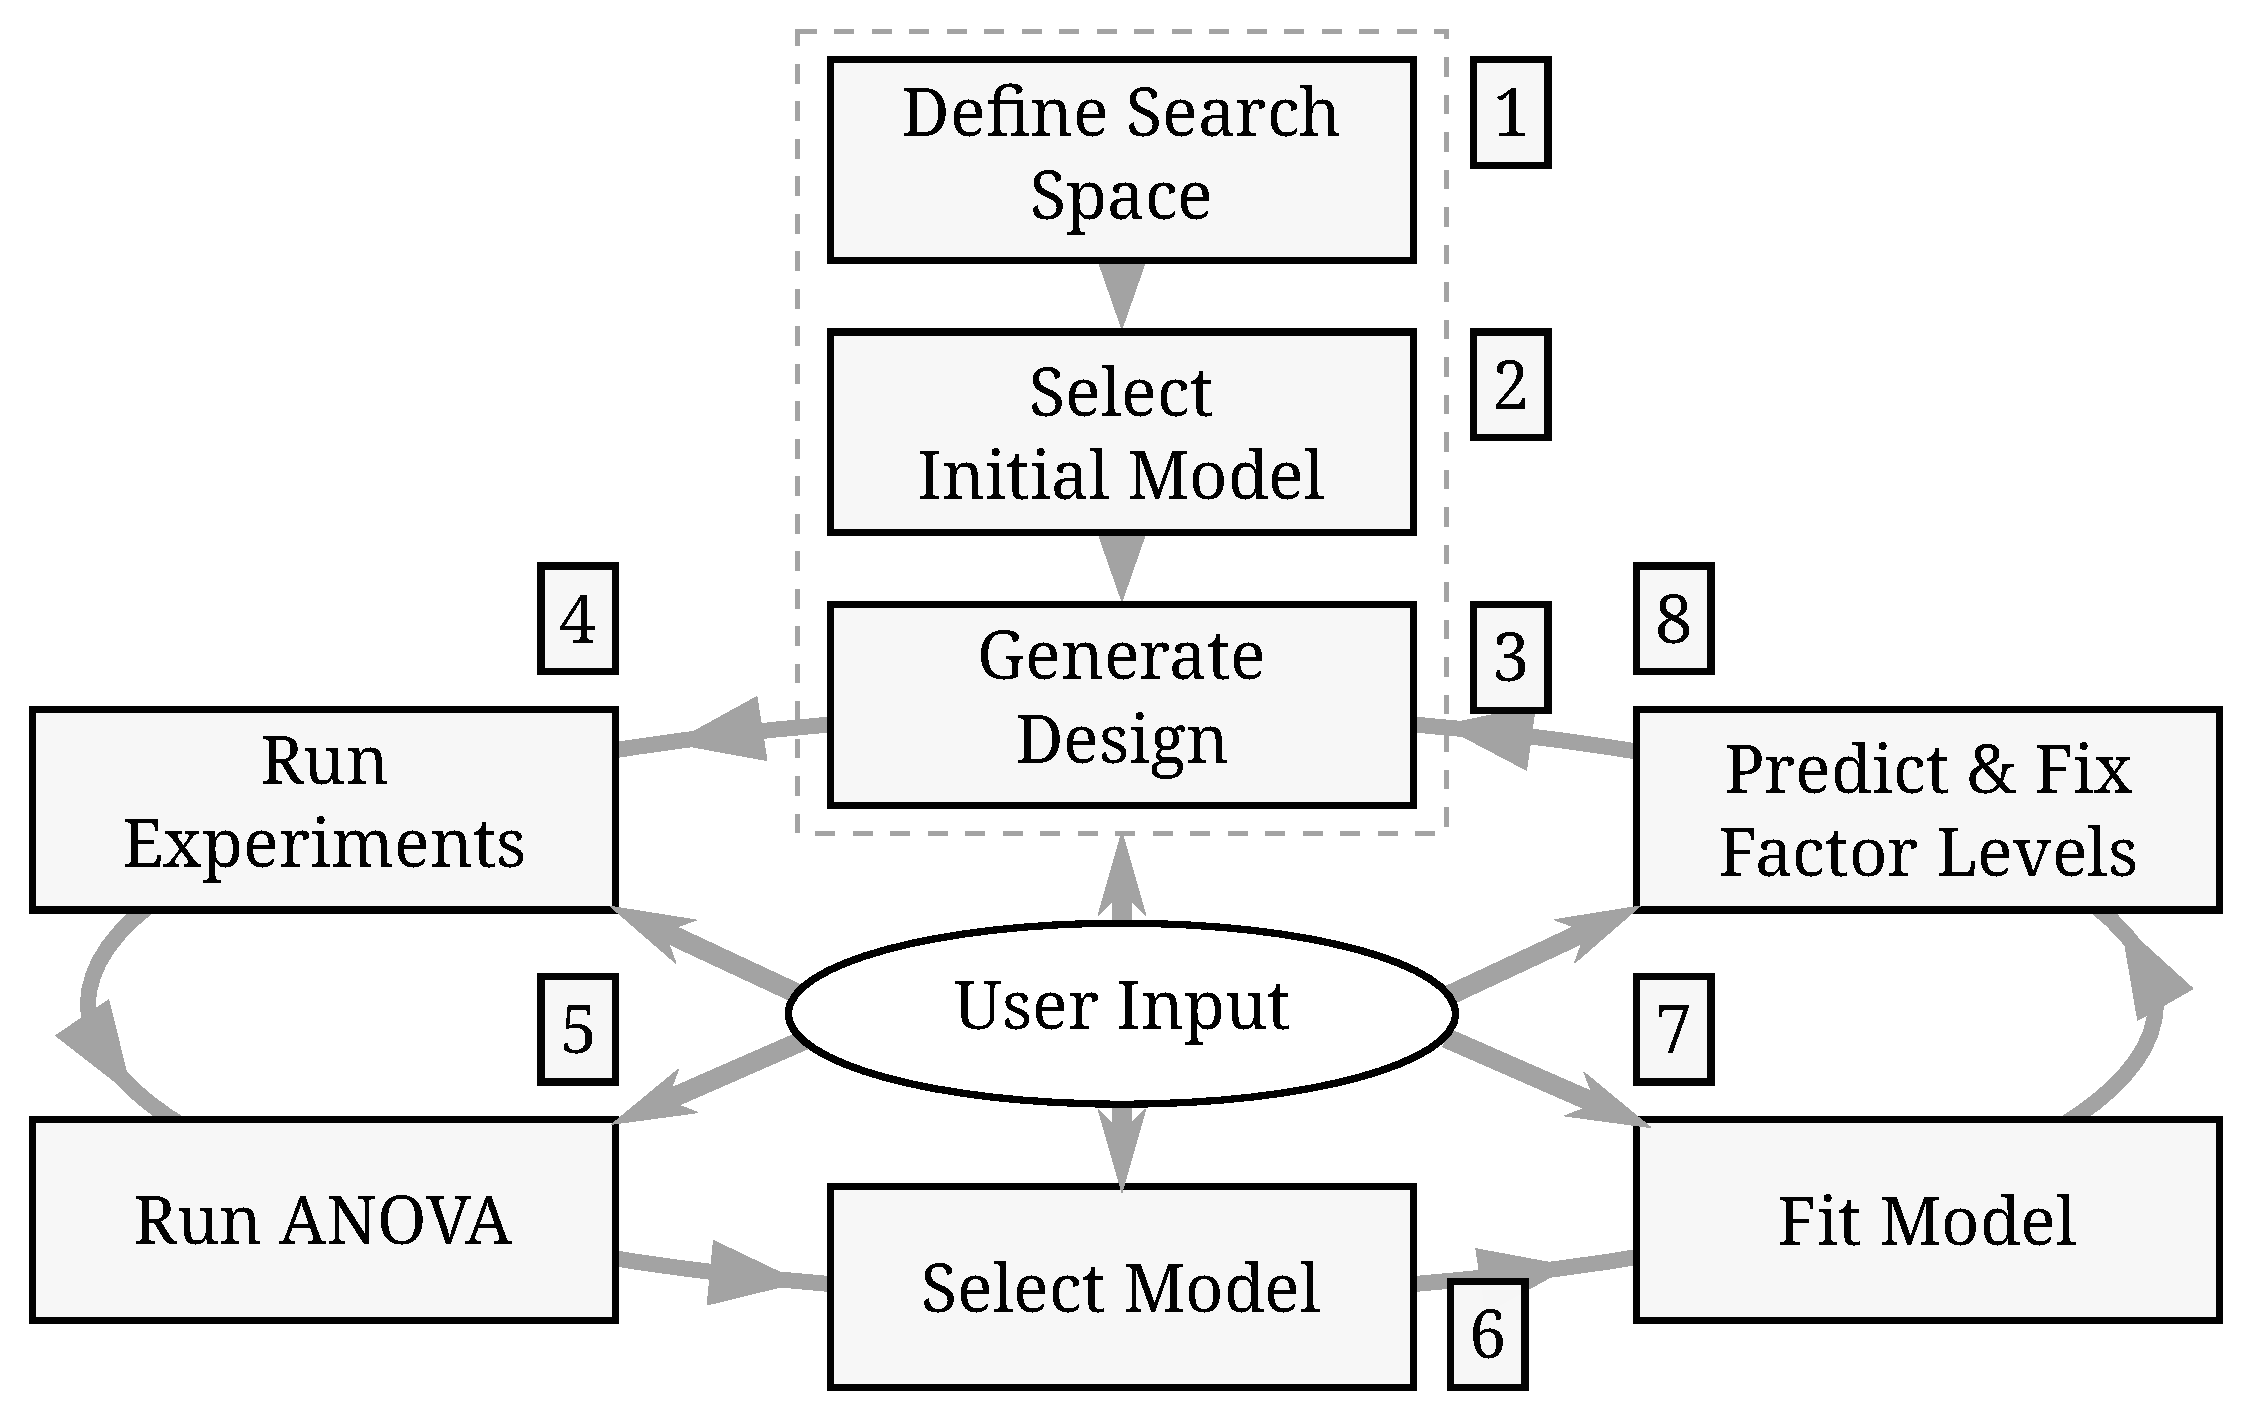
\includegraphics[width=.74\linewidth]{../../../img/doe_anova_strategy.pdf}
\end{center}

\vspace{-.2cm}
\end{center}

\begin{center}
\scriptsize{Autotuning under Tight Budget Constraints: \\ A Transparent Design of Experiments Approach (CCGRID 2019)}
\end{center}
\end{frame}
\section{Results on a GPU Laplacian Kernel}
\label{sec:org8c8128b}
\begin{frame}[label={sec:orgb5fe414}]{GPU Laplacian Kernel: A Motivating Example}
\begin{columns}
\begin{column}{0.5\columnwidth}
\begin{block}{Search Problem}
\begin{itemize}
\item 7 parameters: 6 \alert{numerical}, 1 \alert{boolean}
\item Good starting performance model
\item Measured all 23120 configurations
\item Known \alert{global optimum}
\item Budget of \alert{125 points}
\end{itemize}
\end{block}
\end{column}

\begin{column}{0.5\columnwidth}
\begin{block}{Initial Model}
\footnotesize
\begin{align*}
cost = & \; y\_component\_number + 1 / y\_component\_number \; + \\
& \; vector\_length + lws\_y + 1 / lws\_y \; + \\
& \; load\_overlap + temporary\_size \; + \\
& \; elements\_number + 1 / elements\_number \; + \\
& \; threads\_number + 1 / threads\_number
\end{align*}
\normalsize
\end{block}
\end{column}
\end{columns}

\vspace{-.3cm}

\uncover<2>{
\begin{center}
  \colorbox{Highlight}{\parbox[c]{0.72\textwidth}{\centering We were  always close to
        the \alert{optimum} and used \alert{half of the budget}}}
\end{center}
}

\vspace{-.3cm}

\begin{center}
\begin{center}
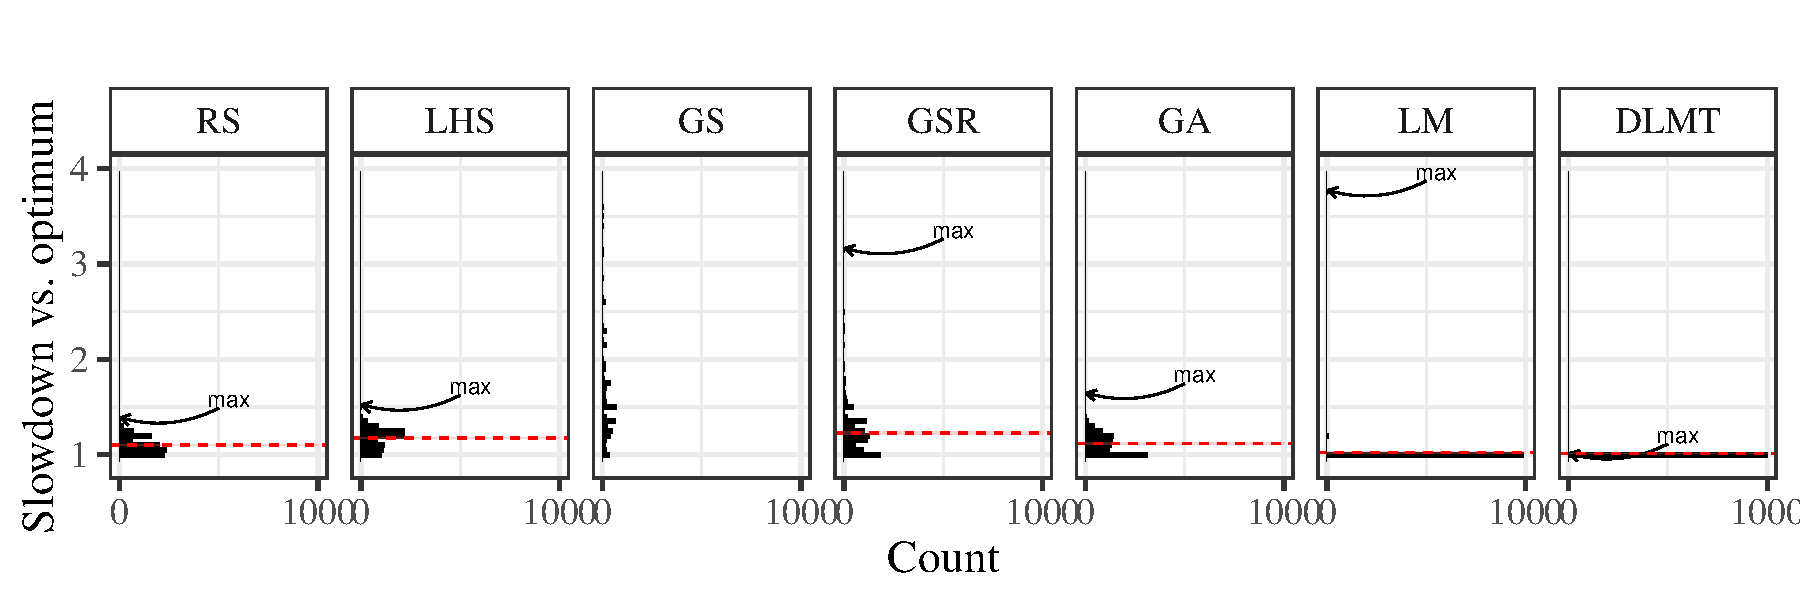
\includegraphics[width=\columnwidth]{../../../img/comparison_histogram.pdf}
\end{center}
\end{center}
\end{frame}
\section{Results on the SPAPT Benchmark}
\label{sec:org407f4f2}
\begin{frame}[label={sec:orgb012e61},fragile]{SPAPT: Search Problems in Automatic Performance Tuning}
 \begin{columns}
\begin{column}{0.41\columnwidth}
\begin{block}{Search Problem}
\begin{itemize}
\item \alert{Orio}: source code transformation
\item Baseline: \texttt{gcc -O3}, no transformations
\item Random sampling (\alert{RS}) vs. D-Optimal approach (\alert{DLMT})
\item 10 repetitions: measure \alert{speedup} and \alert{time-to-solution}
\item Out of 16 kernels:
\begin{itemize}
\item 3 with small impact
\item 6 with similar performance gains
\item \colorbox{Highlight}{7 with \alert{gains found faster}}
\end{itemize}
\end{itemize}
\end{block}
\end{column}
\begin{column}{0.59\columnwidth}
\begin{block}{Search Space}
\vspace{-0.4cm}

\begin{center}
\begin{table}[t]
\label{tab:org9b7608f}
\centering
\scriptsize
\begin{tabular}{llll}
\toprule
Kernel & Operation & Factors & Size\\
\midrule
\texttt{atax} & Matrix transp. \& vector mult. & 18 & \(2.6 \times 10^{16}\)\\
\texttt{dgemv3} & Scalar, vector \& matrix mult. & 49 & \(3.8 \times 10^{36}\)\\
\texttt{gemver} & Vector mult. \& matrix add. & 24 & \(2.6 \times 10^{22}\)\\
\texttt{gesummv} & Scalar, vector, \& matrix mult. & 11 & \(5.3 \times 10^{9}\)\\
\texttt{hessian} & Hessian computation & 9 & \(3.7 \times 10^{7}\)\\
\texttt{mm} & Matrix multiplication & 13 & \(1.2 \times 10^{12}\)\\
\texttt{mvt} & Matrix vector product \& transp. & 12 & \(1.1 \times 10^{9}\)\\
\texttt{tensor} & Tensor matrix mult. & 20 & \(1.2 \times 10^{19}\)\\
\texttt{trmm} & Triangular matrix operations & 25 & \(3.7 \times 10^{23}\)\\
\texttt{bicg} & Subkernel of BiCGStab & 13 & \(3.2 \times 10^{11}\)\\
\texttt{lu} & LU decomposition & 14 & \(9.6 \times 10^{12}\)\\
\texttt{adi} & Matrix sub., mult., \& div. & 20 & \(6.0 \times 10^{15}\)\\
\texttt{jacobi} & 1-D Jacobi computation & 11 & \(5.3 \times 10^{9}\)\\
\texttt{seidel} & Matrix factorization & 15 & \(1.3 \times 10^{14}\)\\
\texttt{stencil3d} & 3-D stencil computation & 29 & \(9.7 \times 10^{27}\)\\
\texttt{correlation} & Correlation computation & 21 & \(4.5 \times 10^{17}\)\\
\bottomrule
\end{tabular}
\end{table}

\scriptsize{Balaprakash P, Wild SM, Norris B. SPAPT: Search problems in automatic performance tuning. Procedia Comp. Sci. 2012 Jan 1;9:1959-68.}
\end{center}
\end{block}
\end{column}
\end{columns}
\end{frame}

\begin{frame}[label={sec:org04fdad3}]{SPAPT: Search Problems in Automatic Performance Tuning}
\begin{center}
\begin{center}
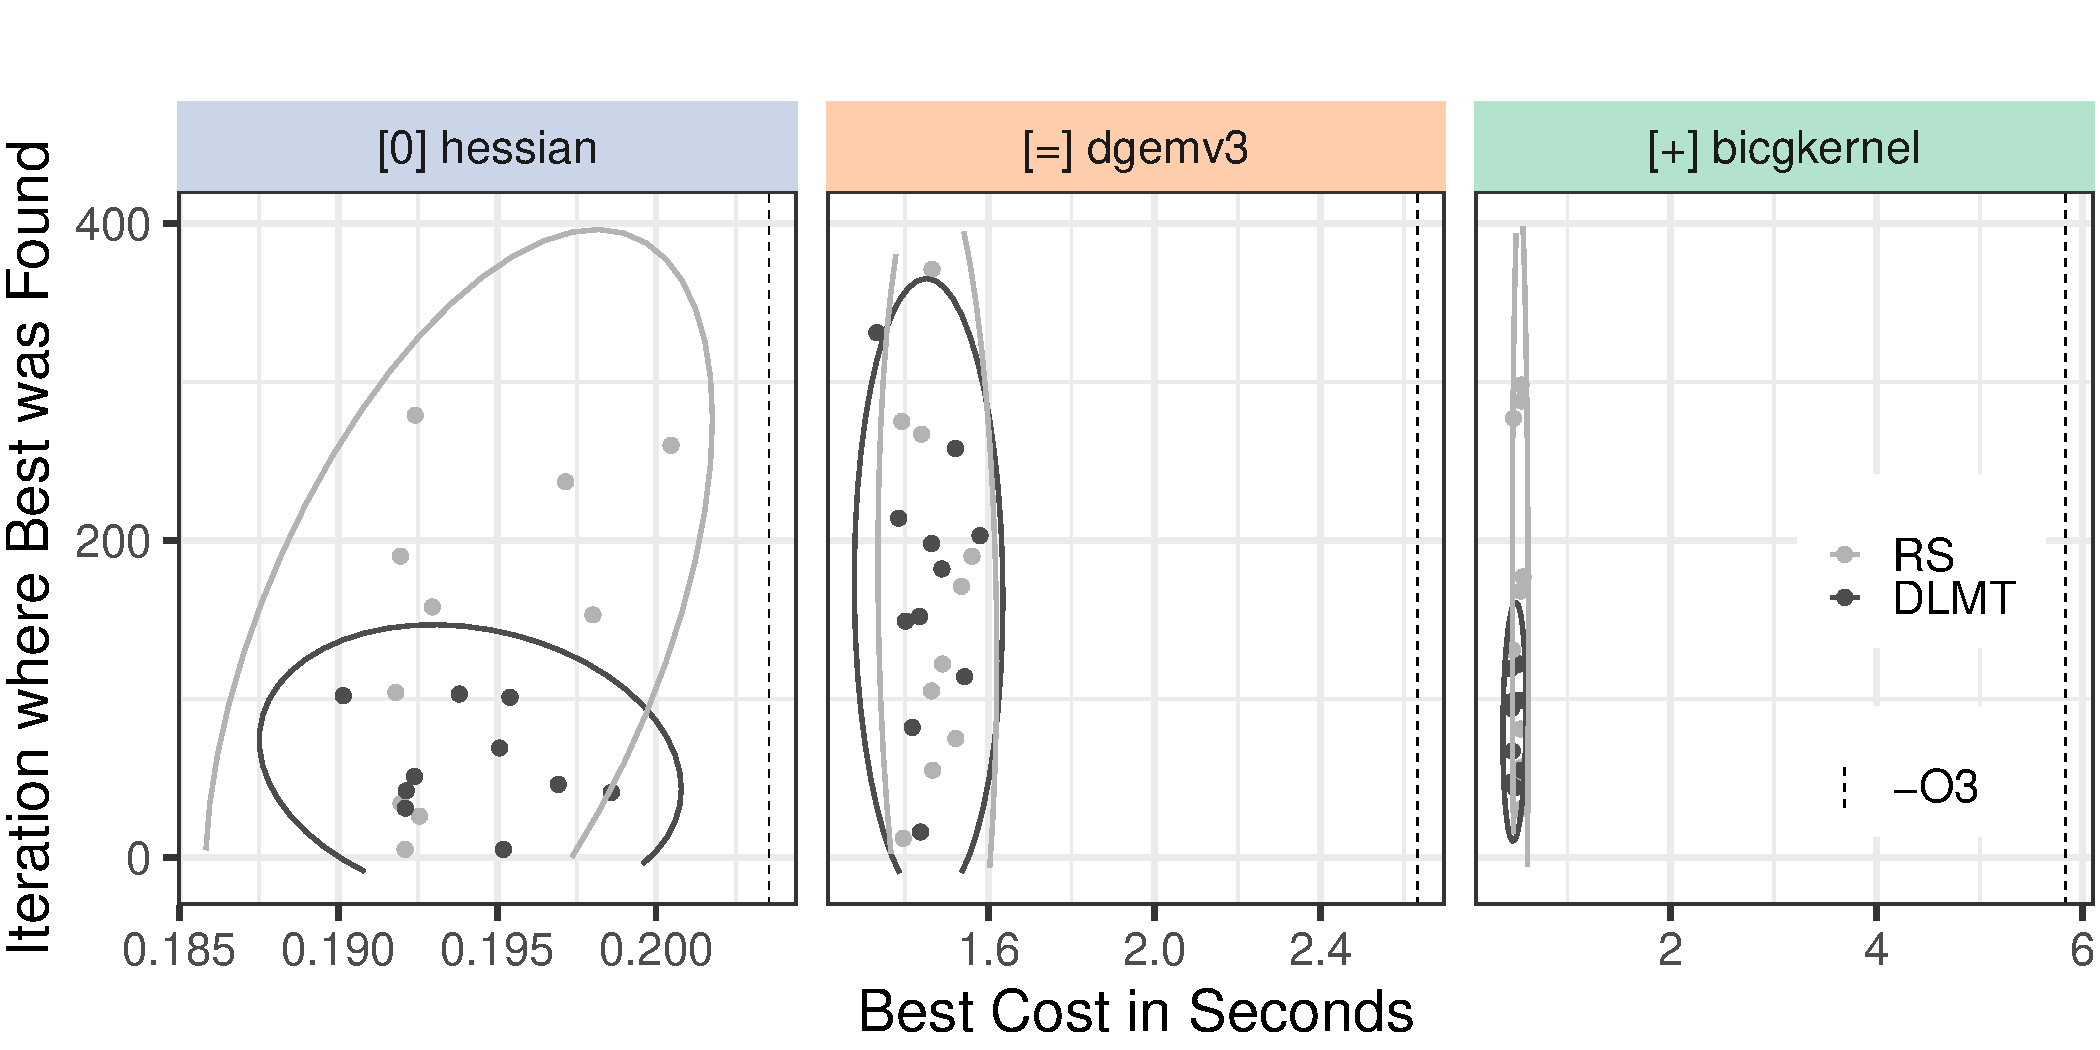
\includegraphics[width=\linewidth]{../../../img/iteration_best_comparison.pdf}
\end{center}
\end{center}
\end{frame}
\begin{frame}[label={sec:orgbfde378}]{SPAPT: Search Problems in Automatic Performance Tuning}
\begin{center}
\begin{center}
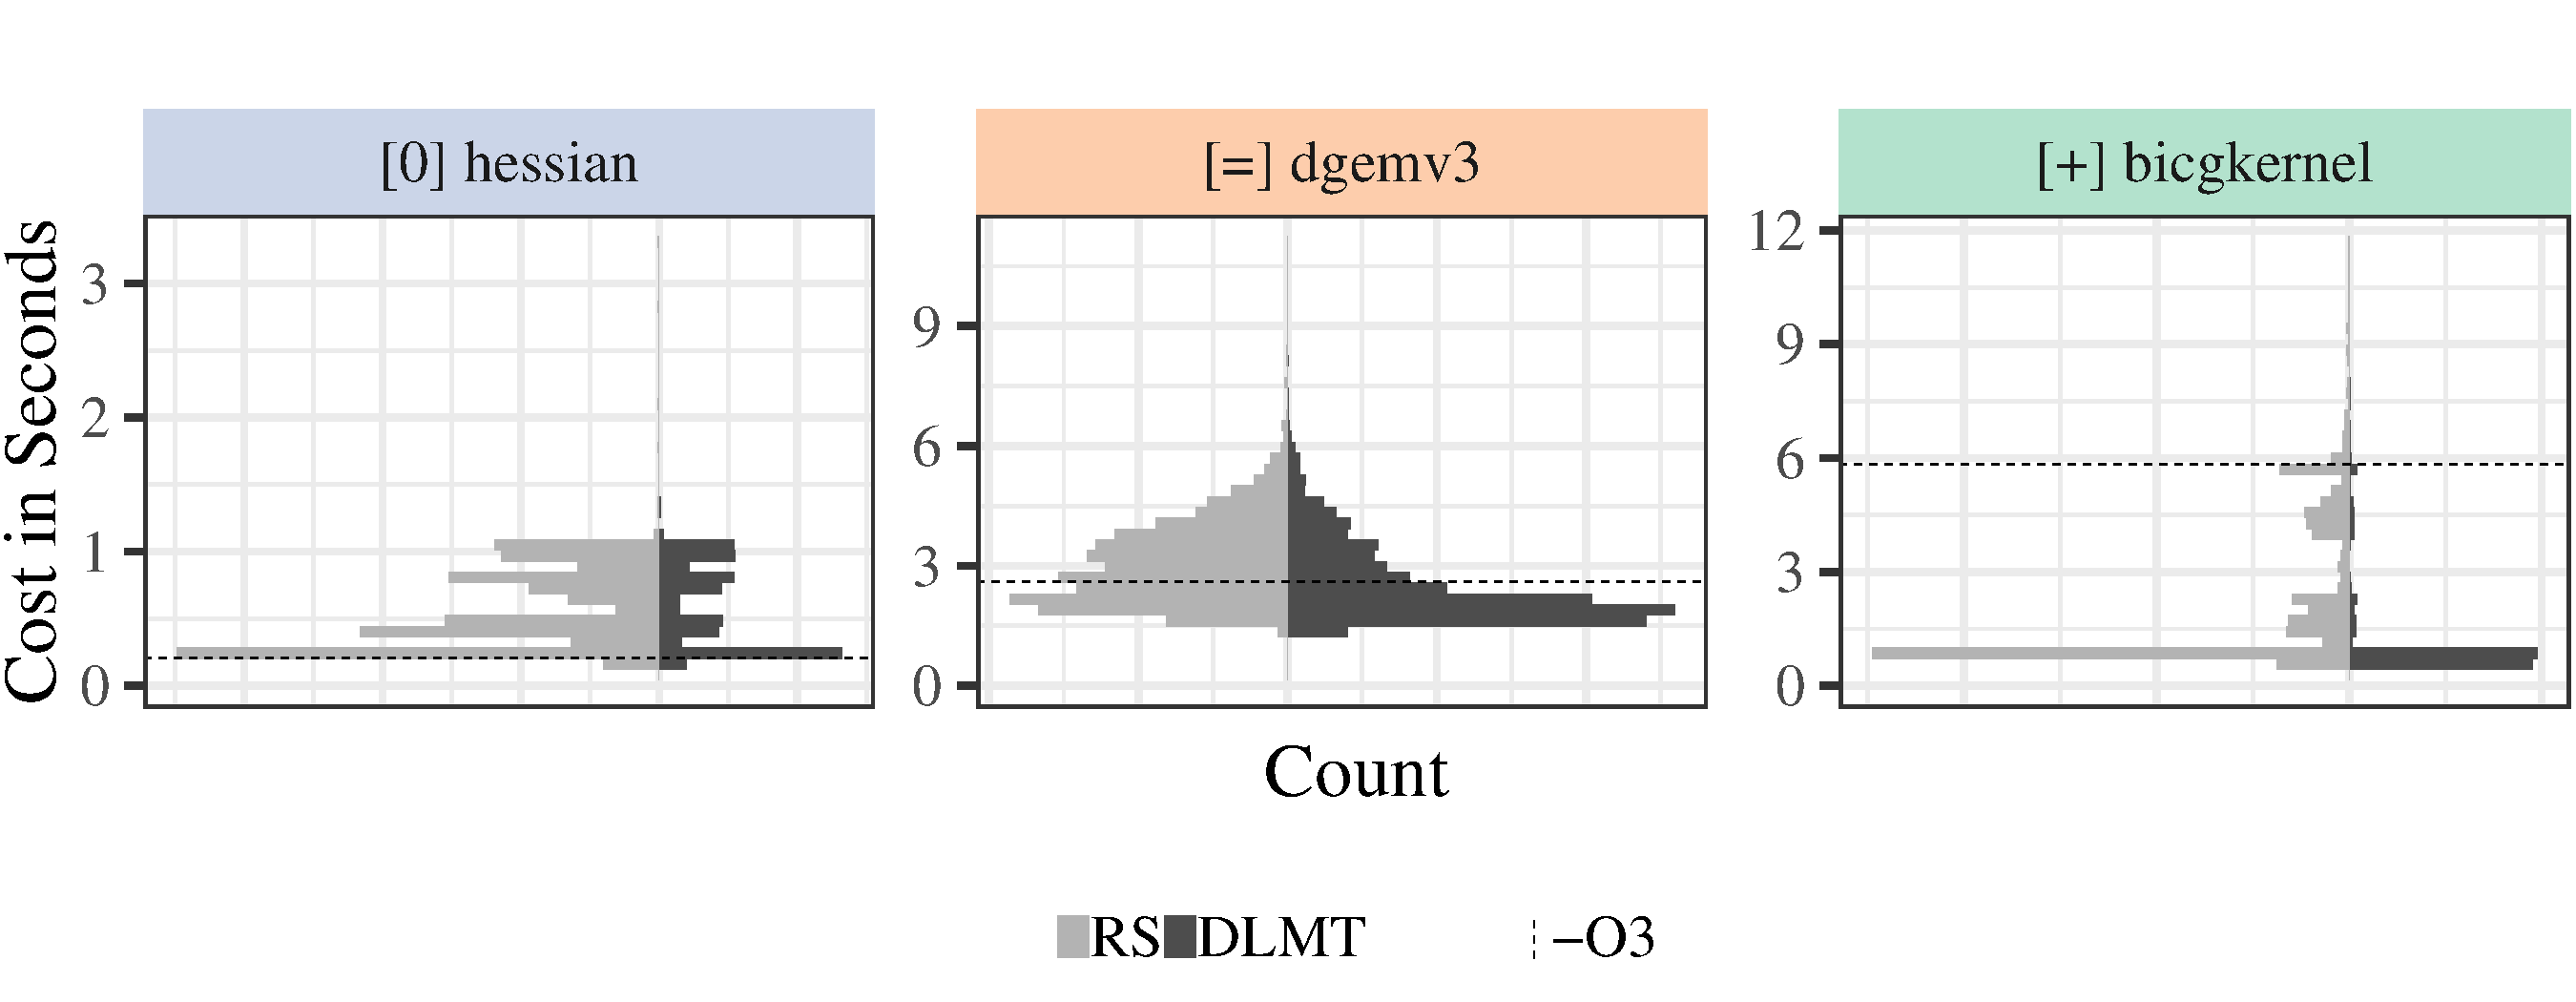
\includegraphics[width=\linewidth]{../../../img/split_histograms.pdf}
\end{center}
\end{center}
\end{frame}
\begin{frame}[label={sec:org310abfe}]{SPAPT: Looking for Structure in \emph{bicgkernel}}
\begin{columns}
\begin{column}{0.5\columnwidth}
\begin{block}{ED Methods for \emph{bicgkernel}}
\alert{Consistently} fixes parameters and levels:
\begin{itemize}
\item Quickly identifies \alert{global} structure
\item Restricts to better sub-regions
\end{itemize}

Further exploration:
\begin{itemize}
\item Certain strong effects \alert{``mask''} others
\item Improving starting model:
\begin{itemize}
\item Cubic terms were not significant
\end{itemize}
\end{itemize}
\end{block}
\end{column}
\begin{column}{0.5\columnwidth}
\only<1>{
\begin{center}
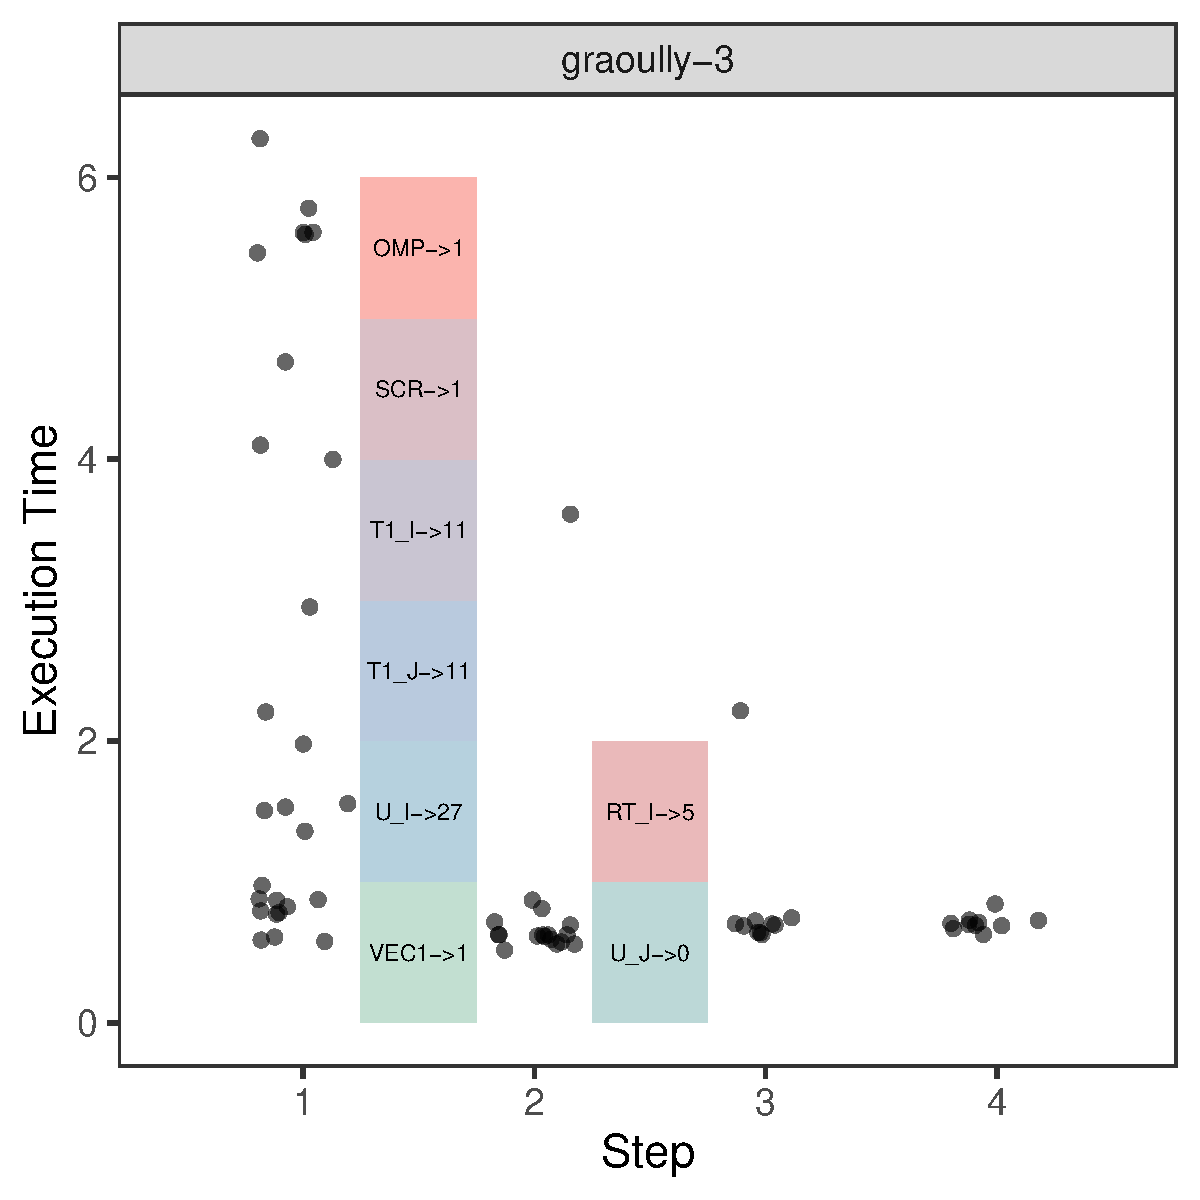
\includegraphics[width=\columnwidth]{../../../img/bicgkernel_factors.pdf}
\end{center}
}
\only<2>{
\begin{center}
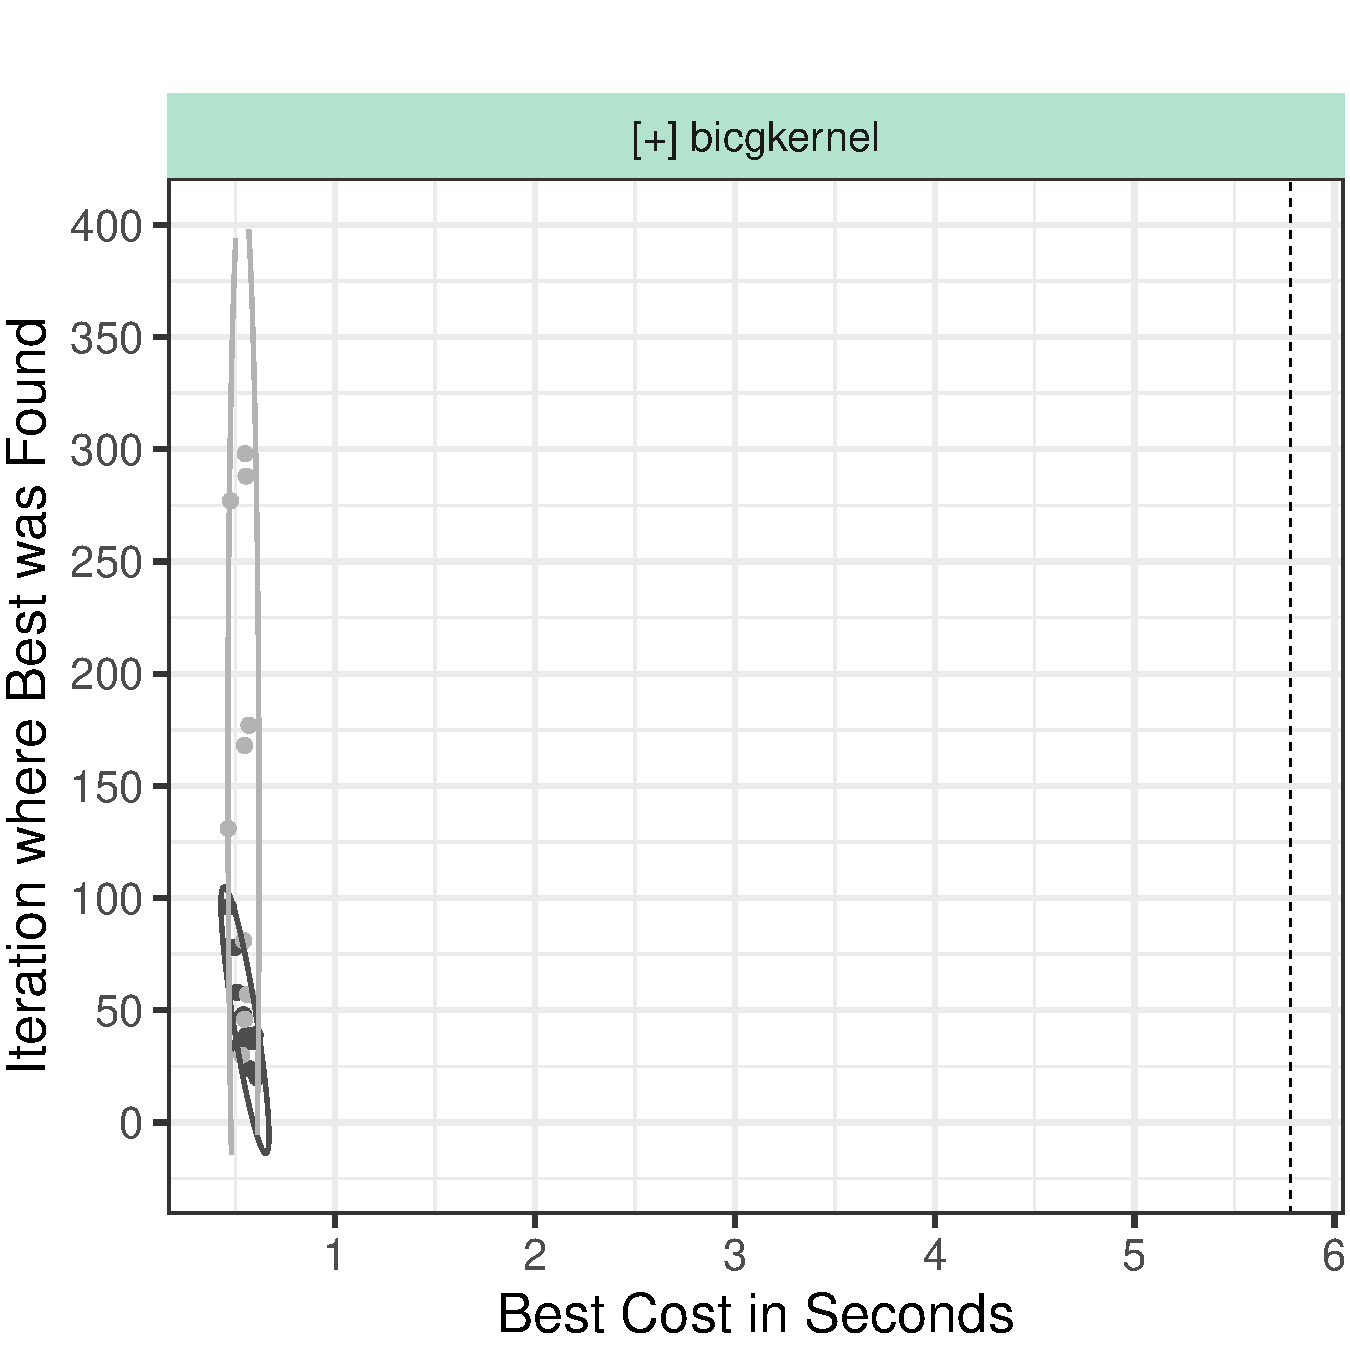
\includegraphics[width=\columnwidth]{../../../img/bicgkernel_updated.pdf}
\end{center}
}
\end{column}
\end{columns}
\end{frame}
\begin{frame}[label={sec:orge5639b7}]{Laplacian and SPAPT kernels Experiments}
With these initial experiments, we showed that:

\begin{columns}
\begin{column}{0.5\columnwidth}
\begin{itemize}
\item Exploiting \alert{global search space structure} helps finding good configurations
fast
\end{itemize}
\end{column}
\begin{column}{0.5\columnwidth}
\begin{itemize}
\item The ED approach is parsimonious, transparent, and \alert{effective} for autotuning
\end{itemize}
\end{column}
\end{columns}
\vspace{0.5cm}
In order  to identify  and exploit \alert{local  structures}, we  need:

\begin{itemize}
\item More \alert{modeling ``flexibility''}
\item \alert{Domain knowledge}
\end{itemize}

\begin{block}{Efforts for Reproducibility}
\begin{center}
\colorbox{Highlight}{\parbox[c]{0.54\textwidth}{\centering \alert{Source code} \& \alert{data} at github.com/phrb/ccgrid19}}
\end{center}
\end{block}
\end{frame}


\section{Gaussian Process Regression}
\label{sec:org1d0d5da}
\begin{frame}[label={sec:org1579b5e}]{Experimental Design with Gaussian Process Regression}
\begin{columns}
\begin{column}{0.5\columnwidth}
\begin{block}{Gaussian Process Regression (GPR)}
\begin{itemize}
\item \alert{Nonparametric}, samples \alert{functions}
\item \alert{Covariance} functions controls priors
\item \alert{Conditions} joint normal probability distributions to \alert{observed data}
\end{itemize}
\begin{block}{Experimental Design with GPR}
\begin{itemize}
\item \colorbox{Highlight}{\alert{Parsimony} \& \alert{Transparency}}
\item \alert{Low-discrepancy} sampling
\item User input to guide optimization
\end{itemize}
\end{block}
\end{block}
\end{column}
\begin{column}{0.5\columnwidth}
\begin{center}
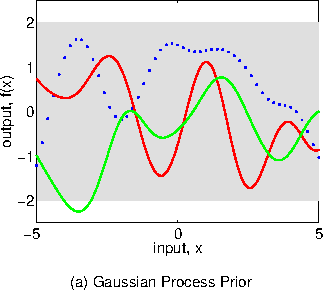
\includegraphics[width=.99\columnwidth]{../../../img/rasmussen_prior.pdf}
\end{center}

\center{\footnotesize
Rasmussen \& Williams, Gaussian Processes \\ for Machine Learning
}
\end{column}
\end{columns}
\end{frame}
\begin{frame}[label={sec:org42fb39a}]{Gaussian Process Regression: Conditioned Posterior}
\begin{center}
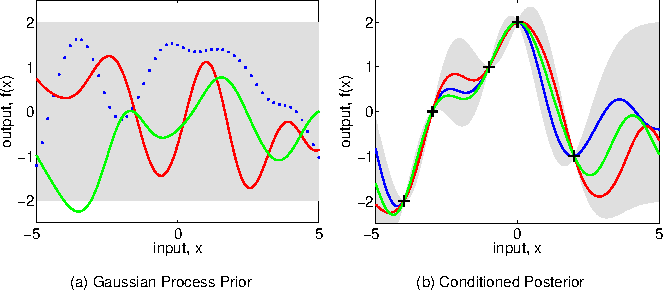
\includegraphics[width=.99\columnwidth]{../../../img/rasmussen_prior_posterior.pdf}
\end{center}

\center{\small
Rasmussen \& Williams, Gaussian Processes  for Machine Learning
}
\end{frame}
\begin{frame}[label={sec:orgf23593d}]{Gaussian Process Regression: Example on a \emph{bickernel} Subspace}
\begin{columns}
\begin{column}{0.5\columnwidth}
\begin{center}
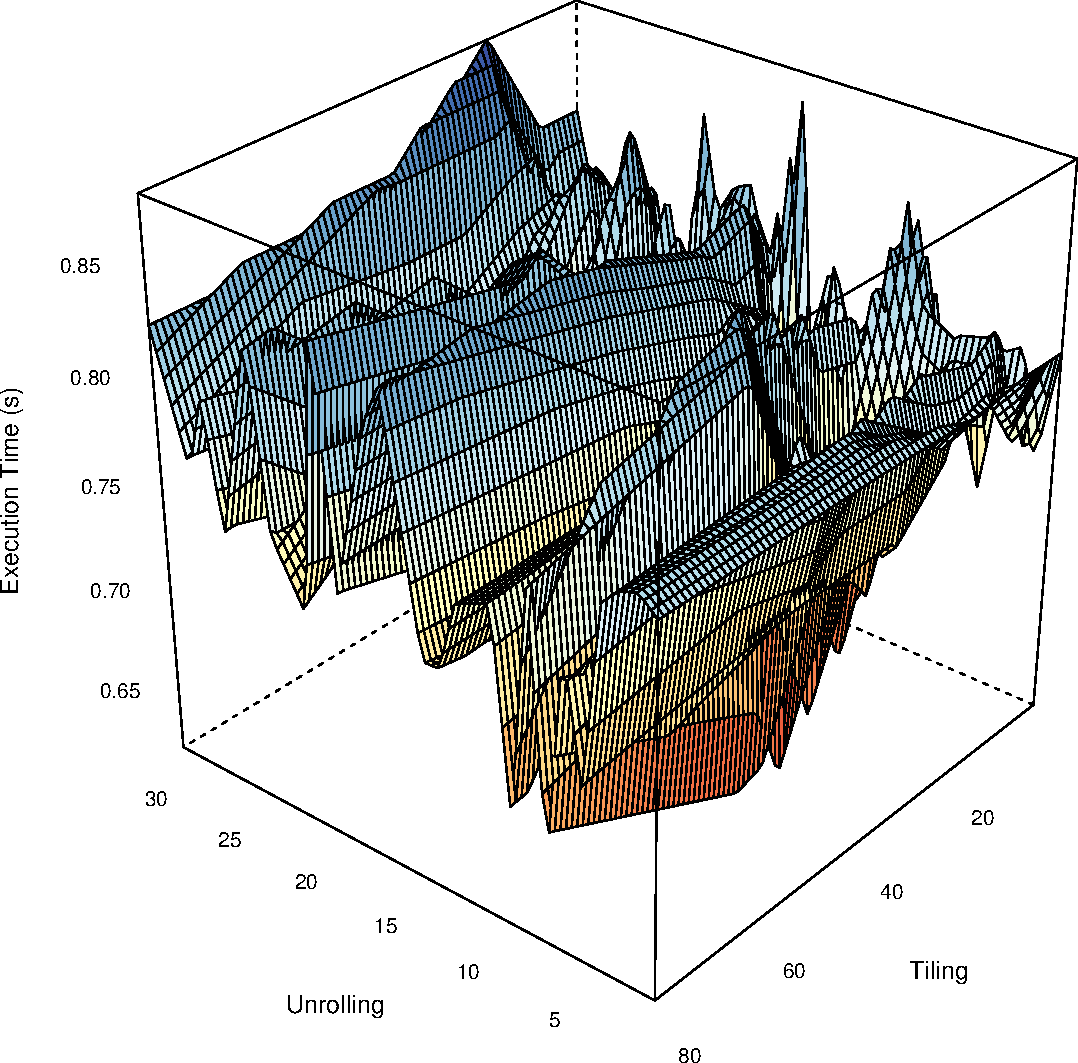
\includegraphics[width=.95\columnwidth]{../../../img/bicgkernel_averaged_search_space.pdf}
\end{center}

\center{\footnotesize
Original \textit{bicgkernel} subspace, \alert{180 points}
}
\end{column}
\begin{column}{0.5\columnwidth}
\only<1>{
\begin{center}
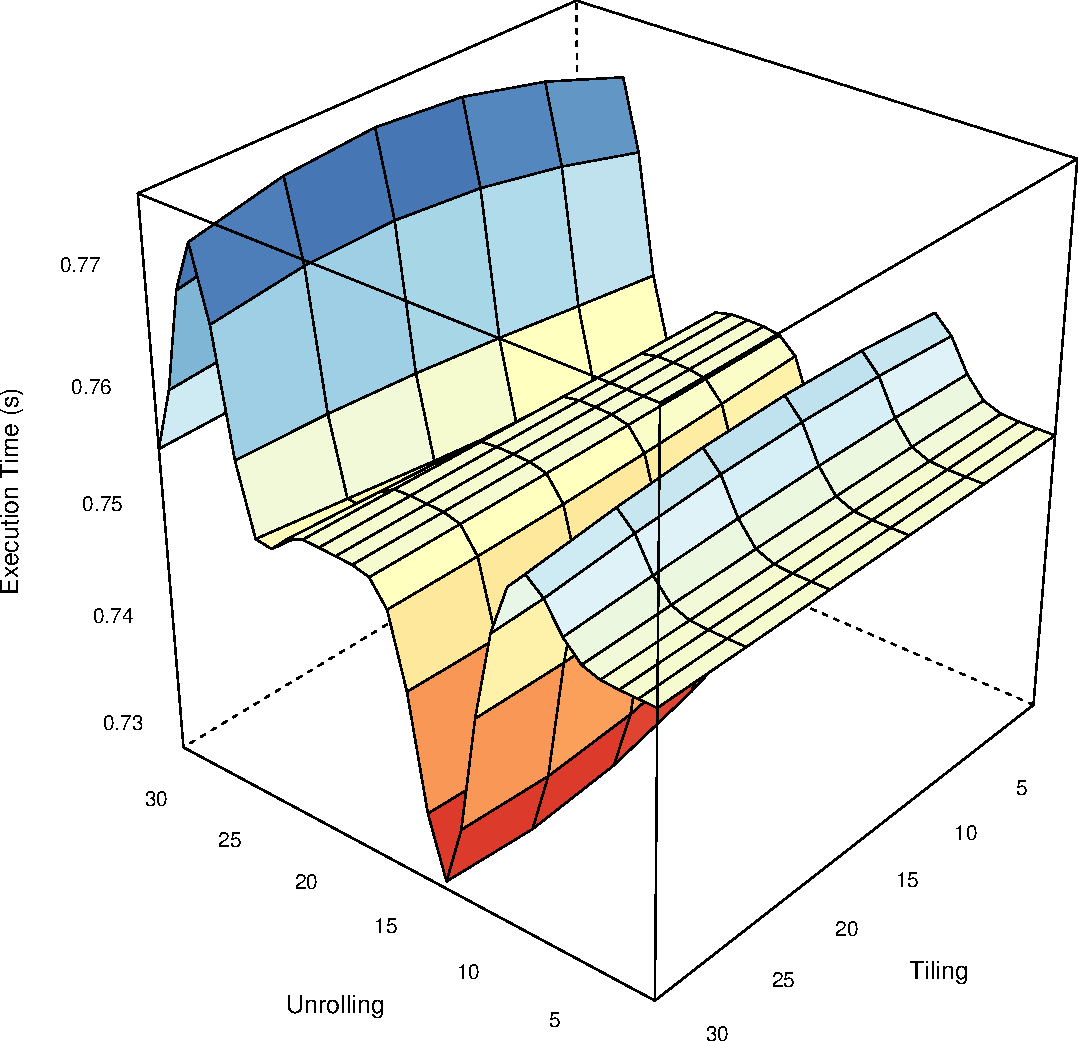
\includegraphics[width=.95\columnwidth]{../../../img/bicgkernel_averaged_search_space_5_pred.pdf}
\end{center}

\center{\footnotesize
Predicted by a Gaussian Process using \alert{5 points}
}
}

\only<2>{
\begin{center}
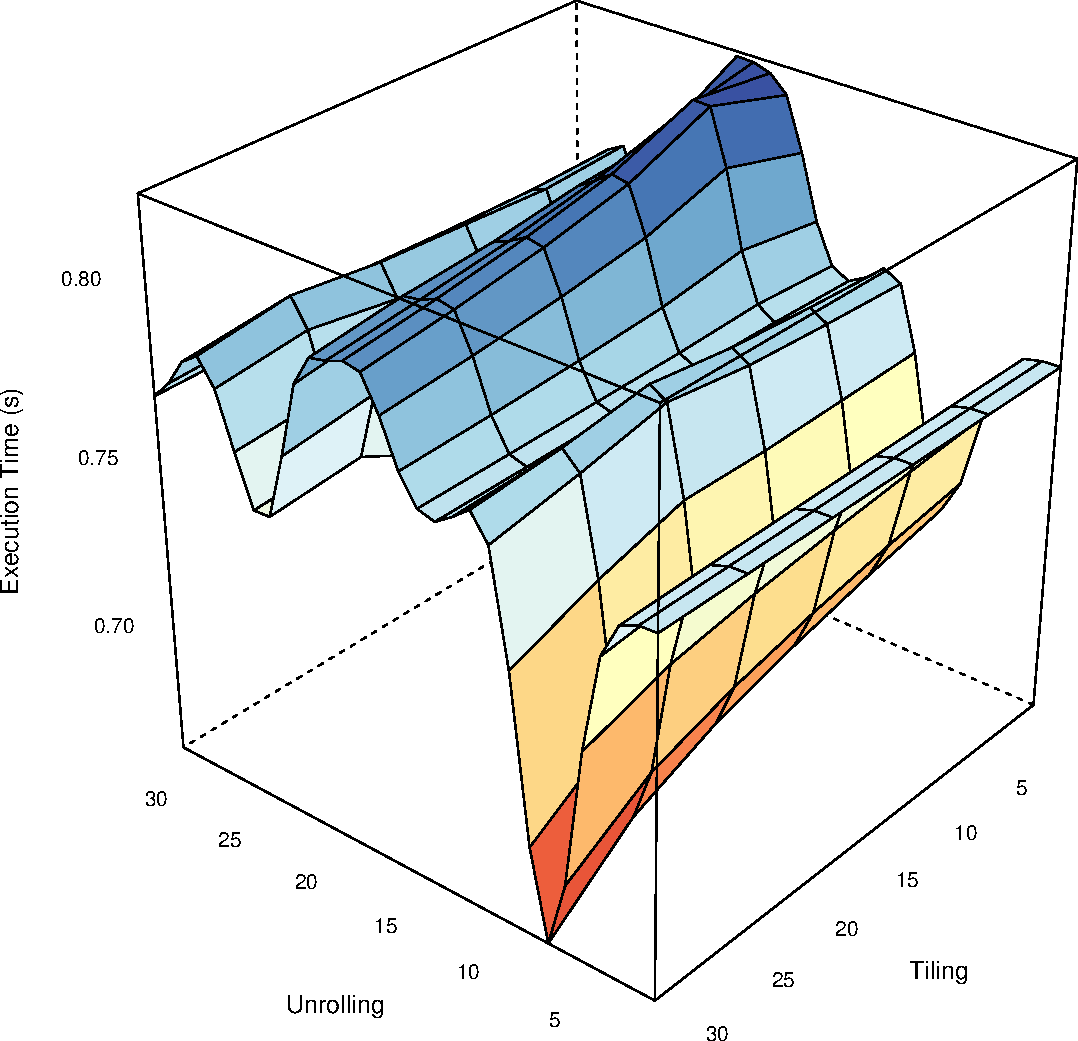
\includegraphics[width=.95\columnwidth]{../../../img/bicgkernel_averaged_search_space_10_pred.pdf}
\end{center}

\center{\footnotesize
Predicted by a Gaussian Process using \alert{10 points}
}
}

\only<3>{
\begin{center}
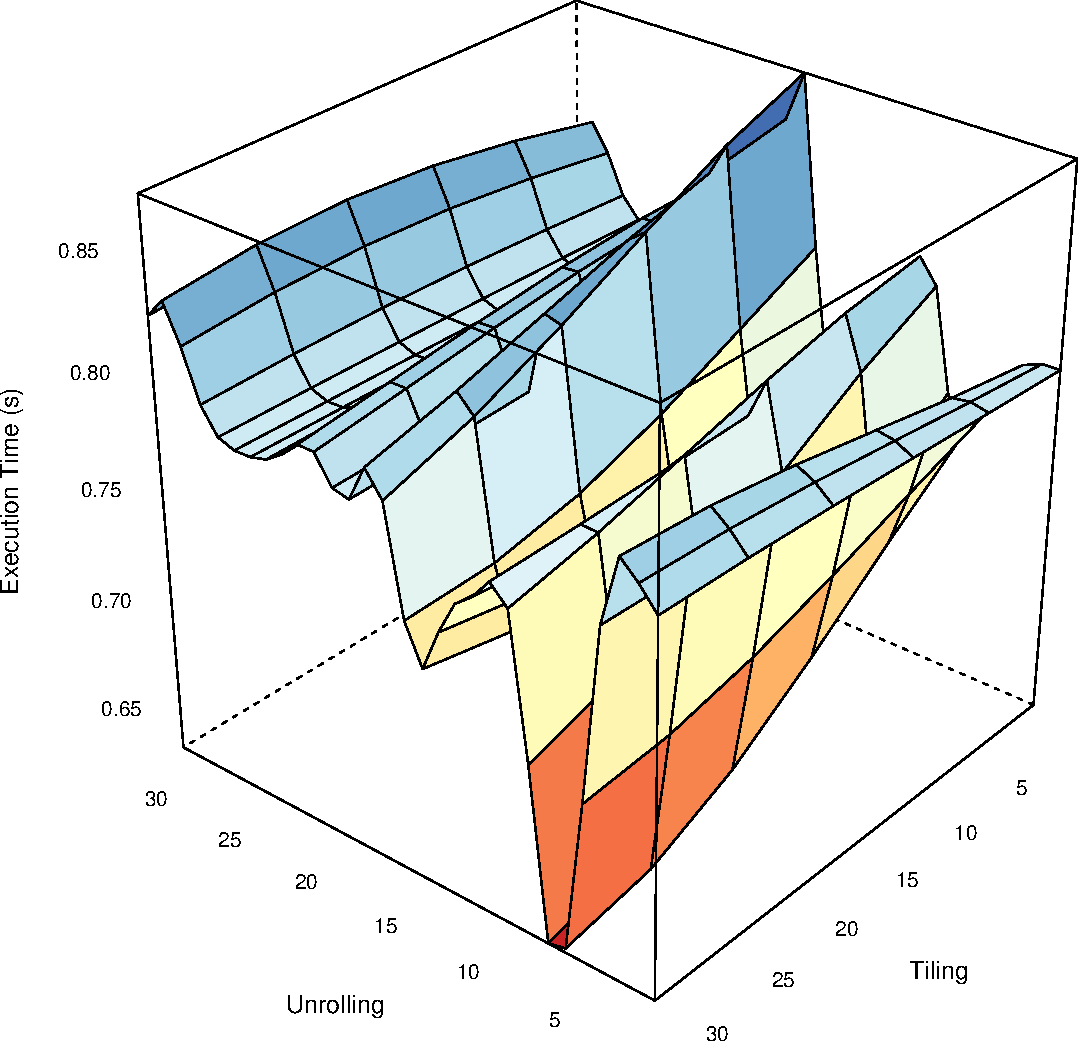
\includegraphics[width=.95\columnwidth]{../../../img/bicgkernel_averaged_search_space_20_pred.pdf}
\end{center}

\center{\footnotesize
Predicted by a Gaussian Process using \alert{20 points}
}
}

\only<4>{
\begin{center}
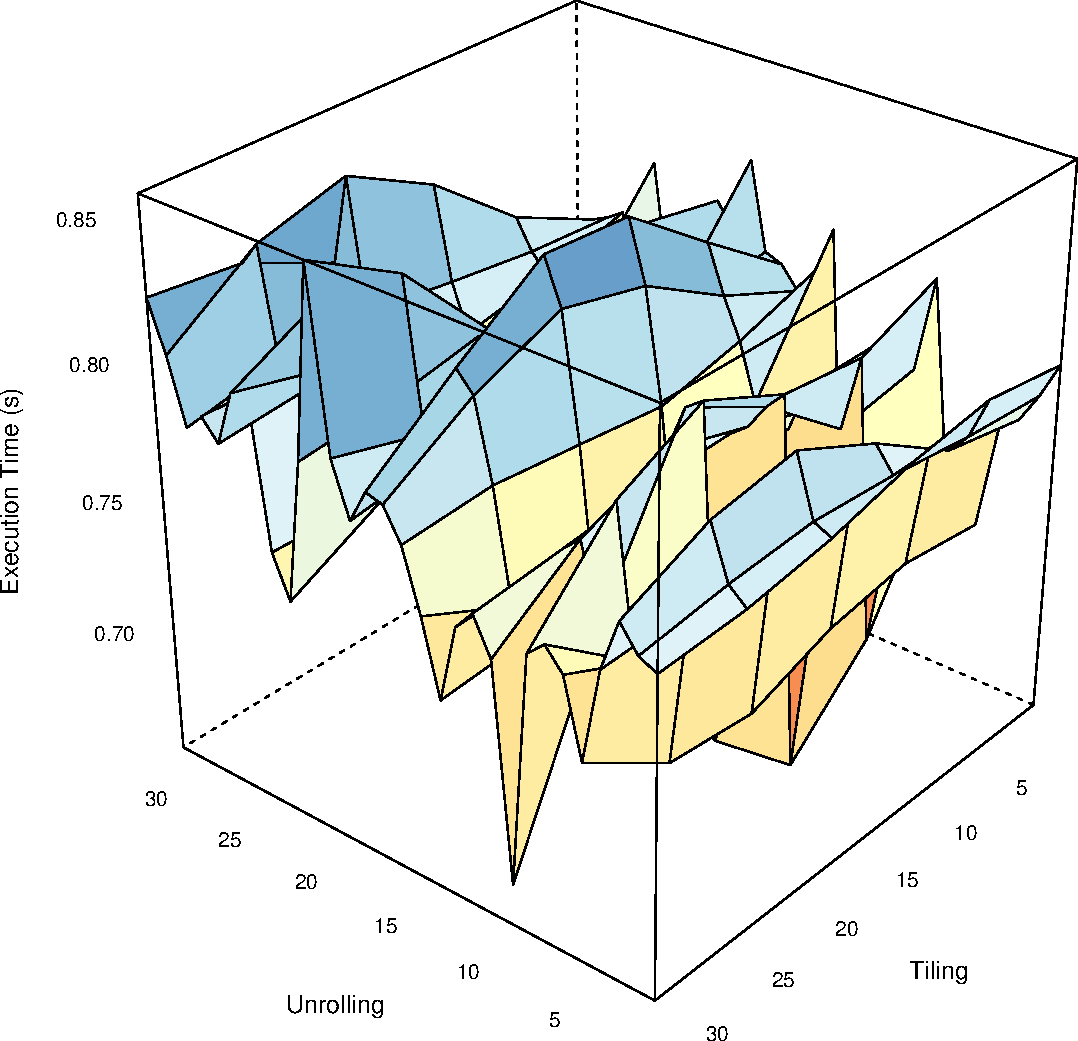
\includegraphics[width=.95\columnwidth]{../../../img/bicgkernel_averaged_search_space_50_pred.pdf}
\end{center}

\center{\footnotesize
Predicted by a Gaussian Process using \alert{50 points}
}
}

\only<5>{
\begin{center}
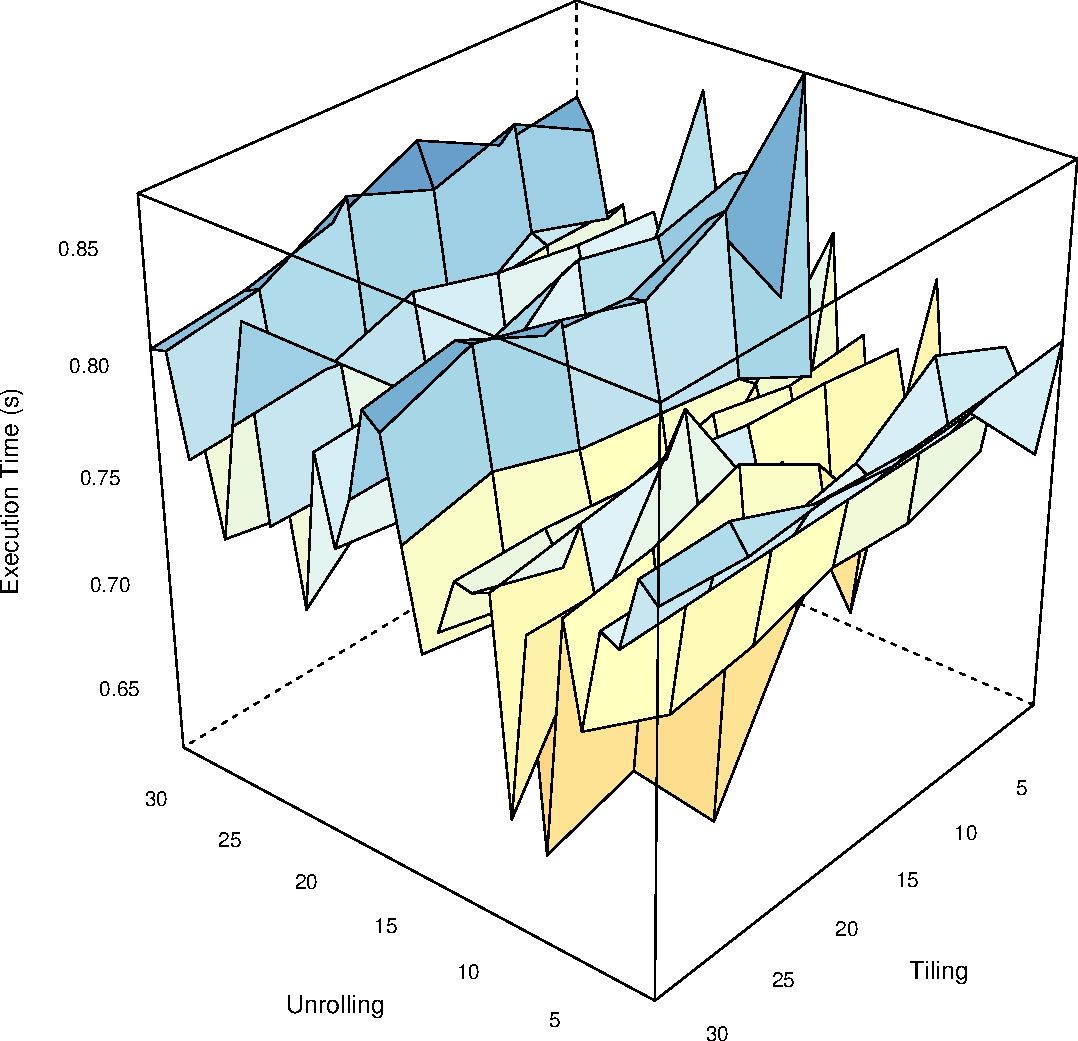
\includegraphics[width=.95\columnwidth]{../../../img/bicgkernel_averaged_search_space_100_pred.pdf}
\end{center}

\center{\footnotesize
Predicted by a Gaussian Process using \alert{100 points}
}
}
\end{column}
\end{columns}
\end{frame}
\begin{frame}[label={sec:org7fc8dc4}]{Gaussian Process Regression: Results on the Complete \emph{bicgkernel} Space}
\begin{center}
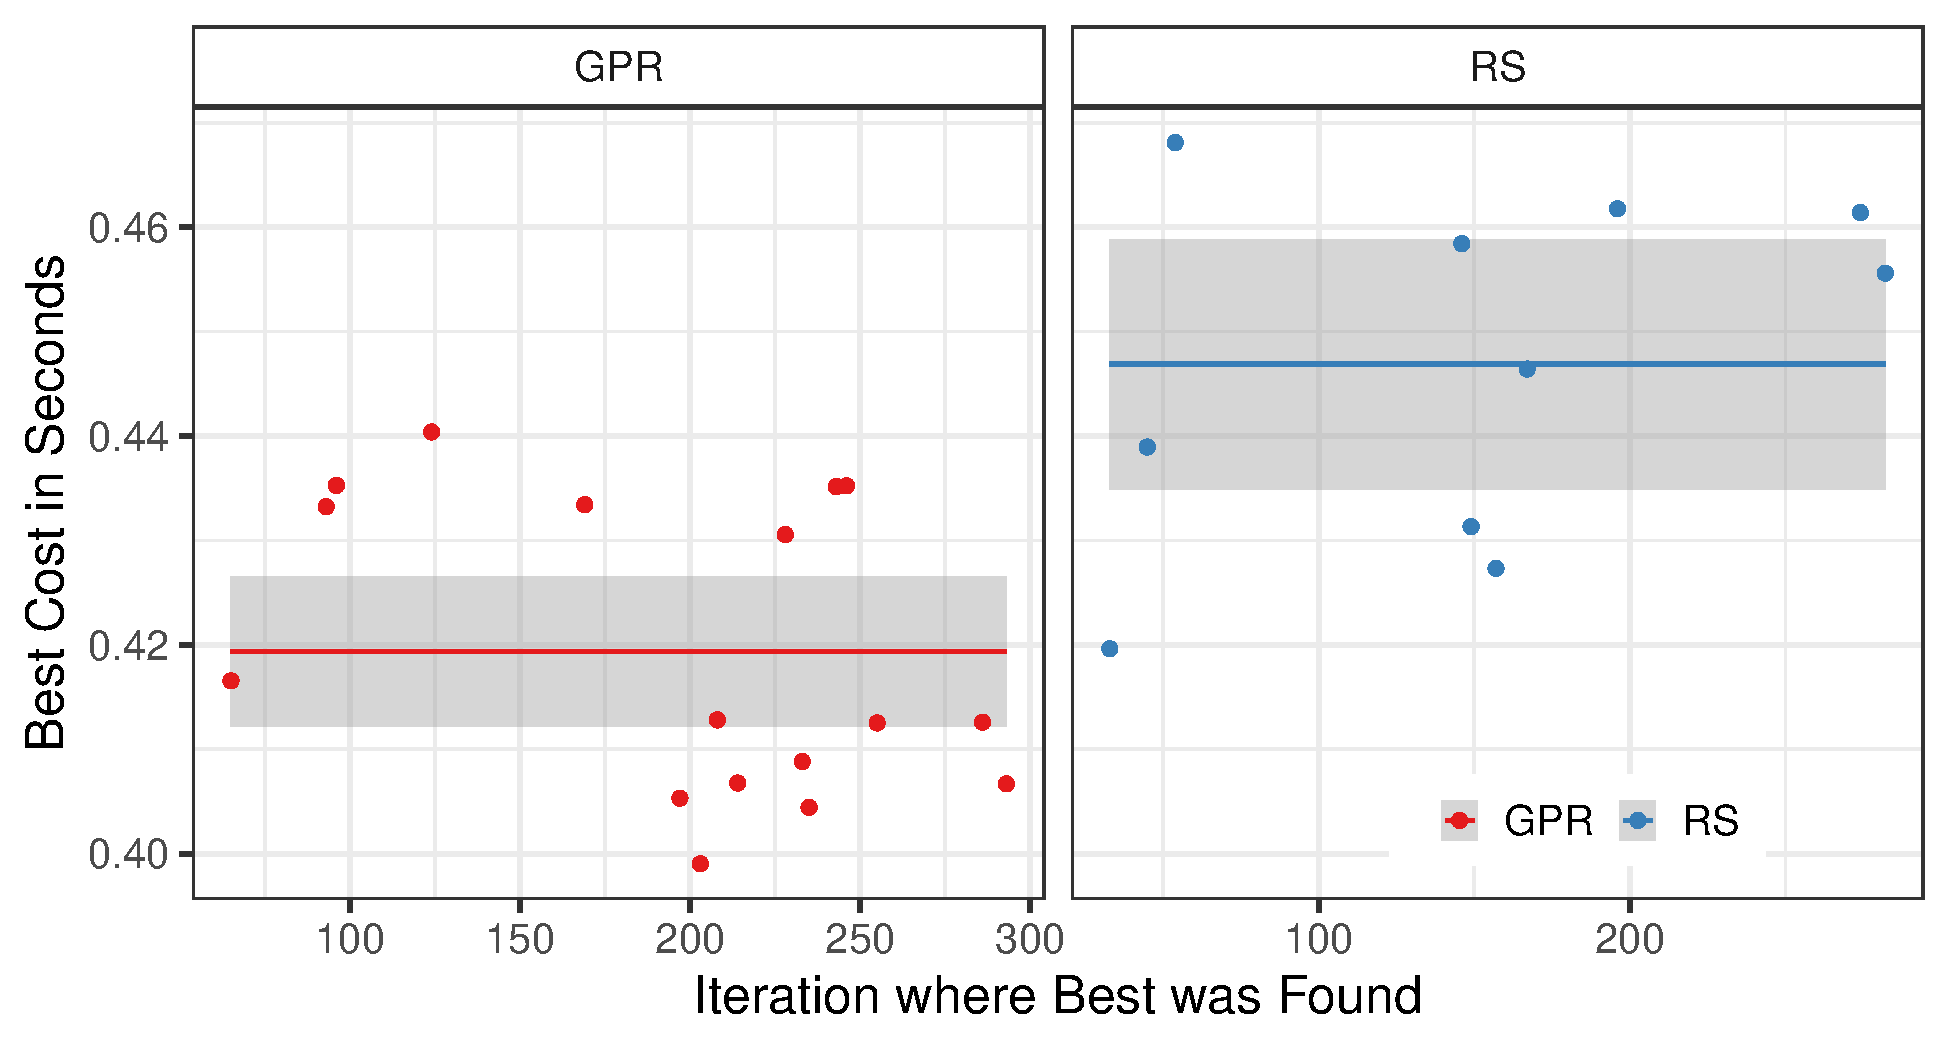
\includegraphics[width=.95\columnwidth]{../../../img/bicgkernel_gpr_results.pdf}
\end{center}
\end{frame}
\section{Next Steps}
\label{sec:org4c79a47}
\begin{frame}[label={sec:org2dd662a}]{Next Steps}
\begin{columns}
\begin{column}{0.5\columnwidth}
\begin{block}{Improving our GPR Approach}
\begin{itemize}
\item Increase sampling on subspaces
\item Choice of \alert{covariance function}, or \alert{kernels}
\item \alert{Flexibility} and \alert{explainability}:
\begin{itemize}
\item Combining kernels
\item Bayesian Information Criterion
\end{itemize}
\end{itemize}
\end{block}
\end{column}
\begin{column}{0.5\columnwidth}
\begin{block}{Apply Experimental Design methods on:}
\begin{itemize}
\item Design space exploration for \alert{quantization} on DNN layers
\item Neural Architecture Search (\alert{NAS}) on CPUs and GPUs
\end{itemize}
\end{block}
\end{column}
\end{columns}
\end{frame}
\maketitle
\end{document}
